\title{\textbf{MinimalPRISM: Spectral Energy-Adaptive Low-Rank Factorization for Efficient Transformer Attention}

\author{Anonymous authors}



\section{Introduction}

\subsection{Motivation}

Transformer-based language models concentrate the majority of their parameters 
in two architectural blocks: the feed-forward network and the multi-head 
self-attention (MHSA) mechanism. In DistilBERT-base, the four attention 
projections $W_Q, W_K, W_V, W_O$ account for approximately \textbf{70\%} of the 
parameters in each transformer block. Reducing the parameter cost of attention 
is therefore a high-leverage compression strategy.

Standard MHSA stores four dense matrices per layer:

\[
W_Q, W_K, W_V, W_O \in \mathbb{R}^{d \times d}
\tag{1.1}
\]

totaling $4d^2$ parameters. For DistilBERT ($d = 768$), this is $4 \times 589{,}824 = 2{,}359{,}296$ 
parameters per layer -- or 14.2M across six layers, a substantial share of the 
66.9M total.

\textbf{Low-rank factorization} is the classical approach. For each $W$, one 
replaces it with a product:

\[
W \approx U V, \qquad
U \in \mathbb{R}^{d_\text{out} \times r}, \quad
V \in \mathbb{R}^{r \times d_\text{in}}, \quad r \ll \min(d_\text{in}, d_\text{out})
\tag{1.2}
\]

The parameter count drops from $d_\text{in} d_\text{out}$ to 
$r(d_\text{in} + d_\text{out})$. The \textbf{reduction factor} is 
$\rho = d_\text{in} d_\text{out} / (r(d_\text{in} + d_\text{out}))$. For square 
matrices at $d = 768$ and $r = 128$: $\rho = 768 / 256 = 3.0$. At $r = 64$: 
$\rho = 6.0$. Classical SVD (Eckart--Young, 1936) gives the optimal rank-$r$ 
approximation in Frobenius norm.

\textbf{The rank-selection problem.} Classical SVD requires choosing $r$ 
a-priori, which is a hard trade-off:

\begin{itemize}
\item \textbf{Too small} -- the approximation error is high, and downstream accuracy
  drops.
\item \textbf{Too large} -- the parameter reduction is minimal, defeating the purpose.

\end{itemize}
In practice, different layers have different \textbf{intrinsic ranks}. Attention 
projections in early layers of DistilBERT tend to have rapidly-decaying 
spectra (effective rank ~30--48), while middle layers decay more slowly 
(effective rank ~80--100). A single global $r$ is suboptimal for both.

\subsection{Problem Statement}

Given a pretrained transformer $\mathcal{M}$ with $N_l$ layers and a target 
energy threshold $\eta \in (0, 1)$, we seek a compressed model 
$\mathcal{M}'$ such that:

\[
\mathcal{M}' \approx \mathcal{M}, \qquad
\frac{|\theta(\mathcal{M}')|}{|\theta(\mathcal{M})|} \ll 1
\tag{1.3}
\]

subject to:

\begin{enumerate}
\item \textbf{Per-layer adaptive rank.} Different layers may use different
  $r_\ell$ chosen automatically.
\item \textbf{Spectral energy preservation.} For each factorized layer,
  $E(r_\ell) \geq \eta$.
\item \textbf{Parameter reduction.} $r_\ell (d_\text{in} + d_\text{out}) < d_\text{in} d_\text{out}$.
\item \textbf{Multi-architecture support.} Flat (DistilBERT), nested (RoBERTa),
  causal with Conv1D (GPT-2), GQA + RoPE (Qwen).
\item \textbf{No base retraining.} Only LoRA adapters may be trained.

\end{enumerate}
\subsection{Our Approach: MinimalPRISM}

\textbf{MinimalPRISM} is a drop-in replacement for the four attention projections 
with three key components:

\begin{enumerate}
\item \textbf{SVD factorization.} Each $W$ is factorized as $U V$ via truncated SVD,
  with $U \in \mathbb{R}^{d_\text{out} \times r_\ell}$ and
  $V \in \mathbb{R}^{r_\ell \times d_\text{in}}$, where $\Sigma^{1/2}$ is
  distributed symmetrically.

\item \textbf{Spectral energy-adaptive rank.} For each weight matrix, compute
  $E(r) = \sum_{i \leq r} \sigma_i^2 / \sum_i \sigma_i^2$ and select:

  $$
  r\_\ell = \min\!\left(r\_\text{max}, \left|\{i : E(i) < \eta\}\right| + 1\right)
  \tag{1.4}
  $$

  This selects the smallest rank that captures at least $\eta$ fraction of
  the spectral energy, capped at $r_\text{max}$.

\item \textbf{LoRA recovery.} After factorization, the base factors $U, V$ are
  frozen and LoRA adapters $A, B$ are added:

  $$
  y = (x V\^{}\top) U\^{}\top + (x A\^{}\top) B\^{}\top \cdot s + b
  \tag{1.5}
  $$

  with $B = 0$ at initialization, so $y$ at step 0 equals the SVD
  approximation.

\end{enumerate}
\textbf{Injection safety.} MinimalPRISM detects nested encoders (RoBERTa) at 
injection time rather than only in weight-copy. It runs a **pre-test on the 
first layer** before mutating the rest of the model, aborting if weight 
extraction fails. This is critical for production correctness.

\subsection{Contributions}

\begin{itemize}
\item \textbf{Energy-adaptive rank selection.} A principled criterion that selects
  a different rank per layer based on spectral decay, avoiding the
  fixed-rank trade-off.
\item \textbf{A safe injection protocol.} Nested-encoder detection at injection time,
  pre-test on the first layer, and strict Frobenius norm validation of
  extracted weights.
\item \textbf{A multi-architecture implementation.} Four families supported
  (DistilBERT, RoBERTa, GPT-2, Qwen3.5) with explicit Conv1D handling, GQA
  support, and RoPE integration.
\item \textbf{A systematic evaluation.} Benchmark on three models on SST-2 with
  ablations over $r_\text{max}$, $\eta$, and LoRA rank.
\item \textbf{Full reproducibility.} Code, checkpoints, and scripts released under
  Apache 2.0.

\end{itemize}
\subsection{Paper Organization}

Section 2 reviews related work. Section 3 provides background. Section 4 
presents MinimalPRISM. Section 5 describes architecture integration. Section 
6 details the setup. Section 7 reports results. Section 8 analyzes 
energy-adaptive behavior. Section 9 discusses guidance. Section 10 lists 
limitations. Section 11 concludes.



\subsection{Notation}

\begin{lstlisting}

---
\end{lstlisting}


\section{Related Work}

\subsection{Low-Rank Matrix Factorization}

\textbf{Classical SVD.} The Eckart--Young theorem (Eckart \& Young, 1936) states 
that the best rank-$r$ approximation of $W$ in Frobenius norm is the 
truncated SVD. MinimalPRISM builds on this foundation.

\textbf{Randomized SVD.} Halko et al. (2011) provide randomized algorithms with 
complexity $\mathcal{O}(dr \log k)$. For our layer sizes, exact SVD is 
feasible within seconds.

\textbf{Weighted low-rank.} Golub et al. (1987) and Srebro \& Jaakkola (2003) study 
weighted variants. Activation-aware methods (Lin et al., 2023; Xiao et al., 
2023) weight the factorization by activation statistics. MinimalPRISM uses 
\textbf{unweighted} SVD but \textbf{adaptive rank}, offering a complementary axis of 
improvement.

\textbf{Tensor decomposition.} Novikov et al. (2015) use tensor-train 
decomposition. MinimalPRISM uses matrix SVD, a simpler primitive.

\subsection{Rank Selection Strategies}

\textbf{Fixed rank.} Most low-rank methods use a fixed global rank (Yu et al., 
2017). This is simple but ignores heterogeneity.

\textbf{Adaptive rank in LoRA.} AdaLoRA (Zhang et al., 2023) learns per-layer 
rank budgets via importance scores. MinimalPRISM uses \textbf{spectral energy}, a 
fixed criterion without learning.

\textbf{Energy-based truncation.} In signal processing, energy-based truncation 
is standard. MinimalPRISM applies it to transformer attention projections.

\subsection{Parameter-Efficient Fine-Tuning}

\textbf{LoRA.} Hu et al. (2021) freeze base weights and train rank-$r$ adapters. 
MinimalPRISM uses LoRA as the recovery mechanism after compression.

\textbf{DoRA.} Liu et al. (2024) decompose weights into magnitude and direction. 
Orthogonal to our work.

\subsection{Attention Variants}

\textbf{Standard MHSA.} Vaswani et al. (2017) introduce the four-projection 
attention. MinimalPRISM preserves the four-projection structure but 
factorizes each.

\textbf{GQA.} Ainslie et al. (2023) use shared KV heads. MinimalPRISM supports 
GQA via \texttt{repeat\_kv} at attention time.

\textbf{MQA.} Shazeer (2019) uses a single KV head. Compatible with our approach.

\subsection{Model Compression}

\begin{table}[H]
\centering
\small
\begin{tabular}{lllll}
\toprule
\textbf{Method} & \textbf{Type} & \textbf{Ratio} & \textbf{Retrain} & \textbf{Calibration} \\
\midrule
DistilBERT & Distillation & 1.6$$\times$ & Yes (from scratch) & -- \\
TinyBERT & Distillation & 7$$\times$ & Yes & -- \\
SparseGPT & Pruning & 2-4$$\times$ & No & Required \\
Wanda & Pruning & 2$$\times$ & No & Required \\
AWQ & Quantization & 4$$\times$ & No & Required \\
GPTQ & Quantization & 4$$\times$ & No & Required \\
A3 & Low-rank + diagonal Fisher & 5$$\times$ & LoRA & Required \\
AASVD & Low-rank + full covariance & 5$$\times$ & LoRA & Required \\
\textbf{MinimalPRISM} & \textbf{Low-rank + spectral energy} & \textbf{50\%$$\times$} & \textbf{LoRA} & \textbf{Not required} \\
\bottomrule
\end{tabular}
\end{table}

\subsection{Position of Our Work}

MinimalPRISM differs from prior work along three axes:

\begin{table}[H]
\centering
\small
\begin{tabular}{lll}
\toprule
\textbf{Axis} & \textbf{Prior} & \textbf{MinimalPRISM} \\
\midrule
\textbf{Rank selection} & Fixed or learned & Spectral energy \\
\textbf{Calibration} & Often required & Not required \\
\textbf{Injection safety} & Rarely pre-tested & Pre-test on first layer \\
\textbf{Nested encoder} & Often broken & Explicit at injection \\
\bottomrule
\end{tabular}
\end{table}

\textbf{Key distinction.} Unlike activation-aware methods (A3, AASVD), MinimalPRISM 
does not require calibration data. Rank is chosen purely from the weight 
spectrum, making it \textbf{training-free} and applicable where calibration data 
is unavailable. Unlike prior SVD methods, MinimalPRISM uses a **per-layer 
adaptive rank**, which requires only the weight matrix, not activations.



\subsection{Comparison Table}

\begin{lstlisting}

---
\end{lstlisting}


\section{Background}

\subsection{Truncated SVD}

For any matrix $W \in \mathbb{R}^{m \times n}$, the SVD is:

\[
W = U \Sigma V^\top
\tag{3.1}
\]

where $U \in \mathbb{R}^{m \times m}$, $V \in \mathbb{R}^{n \times n}$ are 
orthogonal, and $\Sigma$ is diagonal with non-negative entries 
$\sigma_1 \geq \sigma_2 \geq \dots \geq 0$.

\textbf{Truncated SVD} keeps the top-$r$ singular values:

\[
W_r = U_{:, :r} \Sigma_{:r, :r} V_{:r, :}^\top
\tag{3.2}
\]

\textbf{Optimality.} By Eckart--Young, $W_r$ minimizes $\|W - W_r\|_F$ over all 
rank-$r$ matrices. The error:

\[
\|W - W_r\|_F = \sqrt{\sum_{i > r} \sigma_i^2}
\tag{3.3}
\]

\textbf{Symmetric factorization.} We distribute $\Sigma^{1/2}$ between the two 
factors:

\[
U_r = U_{:, :r} \Sigma_{:r, :r}^{1/2}, \qquad
V_r = \Sigma_{:r, :r}^{1/2} V_{:r, :}^\top
\tag{3.4}
\]

so that $W_r = U_r V_r$ with balanced magnitudes.

\subsection{Cumulative Spectral Energy}

Define the \textbf{cumulative spectral energy} of $W$:

\[
E(r) = \frac{\sum_{i=1}^{r} \sigma_i^2}{\sum_{i=1}^{\min(m, n)} \sigma_i^2}
\tag{3.5}
\]

$E(r)$ is monotonically increasing from $E(0) = 0$ to $E(\min(m, n)) = 1$.

\textbf{Effective rank.} Given threshold $\eta$, define:

\[
r_\text{eff}(\eta) = \min\{r : E(r) \geq \eta\}
\tag{3.6}
\]

For rapidly-decaying spectra (e.g., power-law $\sigma_i \propto i^{-2}$), 
$r_\text{eff}$ is small. For uniform spectra, $r_\text{eff}$ approaches 
$\min(m, n)$.

\textbf{Empirical observation.} Transformer weight matrices typically have 
\textbf{power-law or exponential spectral decay}. Empirically, energy thresholds 
of $\eta \in [0.90, 0.99]$ capture the bulk of the spectrum at moderate rank.

\subsection{Multi-Head Self-Attention}

For input $X \in \mathbb{R}^{B \times L \times d}$, MHSA computes:

\[
\begin{aligned}
Q &= X W_Q, \quad K = X W_K, \quad V = X W_V \\
\text{head}_h &= \text{softmax}\!\left(\frac{Q_h K_h^\top}{\sqrt{d_h}}\right) V_h \\
\text{MHSA}(X) &= \text{Concat}(\text{head}_1, \dots, \text{head}_H) W_O
\end{aligned}
\tag{3.7}
\]

MinimalPRISM factorizes each of $W_Q, W_K, W_V, W_O$ independently.

\subsection{Grouped-Query Attention (GQA)}

Modern models use $H_{kv} < H$ KV heads:

\[
K, V \in \mathbb{R}^{B \times L \times H_{kv} d_h}
\tag{3.8}
\]

The KV heads are repeated $H / H_{kv}$ times before attention. MinimalPRISM 
factorizes each at its natural dimension, then applies \texttt{repeat\_kv} during 
forward.

\subsection{Rotary Position Embeddings (RoPE)}

RoPE (Su et al., 2021) rotates $Q, K$ by position-dependent angles:

\[
\tilde{Q}_i = Q_i \cos(\theta_i) + \text{rot}(Q_i) \sin(\theta_i)
\tag{3.9}
\]

MinimalPRISM applies RoPE after projection, preserving the rotational 
structure.

\subsection{LoRA Recovery}

LoRA (Hu et al., 2021) parameterizes:

\[
\Delta W = \frac{\alpha}{r_L} B A
\tag{3.10}
\]

with $A \in \mathbb{R}^{r_L \times d_\text{in}}$, $B \in \mathbb{R}^{d_\text{out} \times r_L}$, 
$B = 0$ at initialization. In MinimalPRISM:

\[
y = (x V^\top) U^\top + (x A^\top) B^\top \cdot s + b
\tag{3.11}
\]

\subsection{Nested Encoder Structure}

In BERT-style models (RoBERTa, BERT), attention is \textbf{nested} inside 
\texttt{BertAttention}:

\begin{lstlisting}
BertAttention
+-- self       (BertSelfAttention)
|   +-- query  (Linear)
|   +-- key    (Linear)
|   +-- value  (Linear)
+-- output     (BertSelfOutput)
    +-- dense  (Linear)   # $\leftarrow$ output projection
\end{lstlisting}

The output projection is \textbf{outside} the inner attention module. When 
replacing the inner attention, the outer \texttt{output.dense} must still apply. 
MinimalPRISM handles this via the \texttt{is\_nested\_encoder} flag, set **at 
injection time** for correctness.

\subsection{Conv1D in GPT-2}

GPT-2 uses HuggingFace's \texttt{Conv1D}, which stores weights as 
\texttt{(in\_features, out\_features)}:

\begin{lstlisting}
class Conv1D(nn.Module):
    def __init__(self, nf, nx):
        self.weight = nn.Parameter(torch.empty(nx, nf))  # (in, out)
\end{lstlisting}

This is \textbf{transposed} relative to \texttt{nn.Linear}. MinimalPRISM detects 
Conv1D via \texttt{hasattr(module, "nf")} and transposes weights before SVD.

\subsection{Notation Summary}

\begin{lstlisting}

---
\end{lstlisting}


\section{Method}

\subsection{Overview}

MinimalPRISM replaces the four attention projections of each transformer 
layer with \textbf{SVD-factorized linear modules}:

\[
W \to (U, V), \qquad
y = (x V^\top) U^\top + \text{LoRA}(x) + b
\tag{4.1}
\]

The factorization is done independently per projection. The rank is chosen 
adaptively per layer based on spectral energy, with a cap at $r_\text{max}$.

\textbf{Figure 4.1} shows the pipeline.

\begin{lstlisting}
   +----------------------------------------------+
   |  Input: pretrained attention module          |
   |  (DistilBERT, RoBERTa, GPT-2, or Qwen)       |
   +--------------------+-------------------------+
                        |
                         
   +----------------------------------------------+
   |  Phase 1: Extraction                          |
   |  Extract W_Q, W_K, W_V, W_O via              |
   |  architecture-specific logic                  |
   +--------------------+-------------------------+
                        |
                         
   +----------------------------------------------+
   |  Phase 2: SVD Factorization (per W)          |
   |  Compute SVD: W = U $\Sigma$ V^T                    |
   |  Compute cumulative energy E(r)              |
   |  r_eff = min(r_max, argmin E(r) $\ge$  )         |
   |  Truncate and symmetrize                     |
   +--------------------+-------------------------+
                        |
                         
   +----------------------------------------------+
   |  Phase 3: Structural Replacement             |
   |  Replace Linear with FactorisedLinear        |
   |  Freeze U, V; add trainable LoRA             |
   +--------------------+-------------------------+
                        |
                         
   +----------------------------------------------+
   |  Output: model with factorized attention     |
   |  Ready for LoRA recovery fine-tuning         |
   +----------------------------------------------+
\end{lstlisting}

\subsection{The `FactorisedLinear` Module}

\subsubsection{Forward Pass}

The module computes:

\[
y = \text{up}(\text{down}(x)) + \text{LoRA}(x)
\tag{4.2}
\]

where:

\begin{itemize}
\item \texttt{down: nn.Linear(d\_in, r, bias=False)} -- stores $V_r \in \mathbb{R}^{r \times d_\text{in}}$
\item \texttt{up: nn.Linear(r, d\_out, bias=True)} -- stores $U_r \in \mathbb{R}^{d_\text{out} \times r}$
\item \texttt{LoRA(x) = (x A\^{}\top) B\^{}\top \cdot s} -- optional adapter

\end{itemize}
\subsubsection{Parameter Count}

\begin{table}[H]
\centering
\small
\begin{tabular}{ll}
\toprule
\textbf{Configuration} & \textbf{Parameters} \\
\midrule
Original \texttt{nn.Linear} & $d_\text{in} d_\text{out}$ \\
\texttt{FactorisedLinear} at rank $r$ & $r(d_\text{in} + d_\text{out})$ \\
\texttt{FactorisedLinear} + LoRA($r_L$) & $r(d_\text{in} + d_\text{out}) + r_L(d_\text{in} + d_\text{out})$ \\
\bottomrule
\end{tabular}
\end{table}

\textbf{Example} for a $768 \times 768$ projection:

\begin{table}[H]
\centering
\small
\begin{tabular}{lll}
\toprule
\textbf{Config} & \textbf{Params} & \textbf{Ratio} \\
\midrule
Original & 589,824 & 1.00$$\times$ \\
r=64 & 98,304 & \textbf{6.00$$\times$} \\
r=128 & 196,608 & 3.00$$\times$ \\
r=64 + LoRA r=16 & 122,880 & 4.80$$\times$ \\
\bottomrule
\end{tabular}
\end{table}

\subsection{Spectral Energy-Adaptive Rank Selection}

\subsubsection{Algorithm}

Given weight $W$ and hyperparameters $r_\text{max}$ (cap) and $\eta$ (energy):

\begin{enumerate}
\item Compute SVD: $W = U \Sigma V^\top$.
\item Compute cumulative energy:
  $$
  E(r) = \frac{\sum\_{i=1}\^{}{r} \sigma\_i\^{}2}{\sum\_i \sigma\_i\^{}2}
  \tag{4.3}
  $$
\item Find the smallest $r$ with $E(r) \geq \eta$:
  $$
  r\_\text{energy} = \left|\{i : E(i) < \eta\}\right| + 1
  \tag{4.4}
  $$
\item Cap the rank:
  $$
  r\_\text{eff} = \min(r\_\text{max}, r\_\text{energy}, \min(d\_\text{in}, d\_\text{out}))
  \tag{4.5}
  $$

\end{enumerate}
\subsubsection{Why Energy?}

The energy criterion captures \textbf{how concentrated the spectrum is}. Two 
extreme cases:

\begin{itemize}
\item \textbf{Rank-1 matrix} ($\sigma_1 > 0$, $\sigma_{i>1} = 0$): $r_\text{energy} = 1$
  for any $\eta > 0$. Very compressible.
\item \textbf{Identity matrix} ($\sigma_i = 1$): $E(r) = r / d$, so
  $r_\text{energy} = \lceil \eta d \rceil$. Less compressible.

\end{itemize}
Real transformer weights lie between these extremes, with power-law or 
exponential decay. The energy criterion adapts to each matrix's spectrum.

\subsubsection{Comparison to Fixed Rank}

\begin{table}[H]
\centering
\small
\begin{tabular}{lll}
\toprule
\textbf{Criterion} & \textbf{Pros} & \textbf{Cons} \\
\midrule
Fixed rank & Simple & Ignores heterogeneity \\
Energy & Adaptive & No task-specific calibration \\
Fisher-weighted & Task-aware & Requires calibration \\
\bottomrule
\end{tabular}
\end{table}

MinimalPRISM uses energy: \textbf{training-free} and applicable wherever the 
model weights are available.

\subsection{Weight Factorization}

\subsubsection{Symmetric Distribution}

We distribute $\Sigma^{1/2}$ between the two factors:

\[
U_r = U_{:, :r} \Sigma_{:r, :r}^{1/2}, \qquad
V_r = \Sigma_{:r, :r}^{1/2} V_{:r, :}^\top
\tag{4.6}
\]

This gives $W_r = U_r V_r$ with balanced factor magnitudes, improving 
training stability (both factors have unit spectral norm up to constants).

\subsubsection{Storage}

The framework stores $V_r$ in \texttt{down.weight} and $U_r$ in \texttt{up.weight}:

\begin{lstlisting}
self.down.weight.data[:r, :] = V_r    # (r, d_in)
self.up.weight.data[:, :r] = U_r      # (d_out, r)
\end{lstlisting}

For $r < \text{target rank}$, remaining rows/columns are zero.

\subsection{Weight Transfer from Pretrained Attention}

MinimalPRISM extracts $W_Q, W_K, W_V, W_O$ from the pretrained attention 
module. This is nontrivial because different architectures store them 
differently.

\subsubsection{Extraction Path (per architecture)}

\begin{table}[H]
\centering
\small
\begin{tabular}{lllll}
\toprule
\textbf{Architecture} & \textbf{$W_Q$} & \textbf{$W_K$} & \textbf{$W_V$} & \textbf{$W_O$} \\
\midrule
DistilBERT & \texttt{q\_lin} & \texttt{k\_lin} & \texttt{v\_lin} & \texttt{out\_lin} \\
RoBERTa & \texttt{self.query} & \texttt{self.key} & \texttt{self.value} & \texttt{output.dense} \\
GPT-2 & \texttt{c\_attn[:d]} & \texttt{c\_attn[d:2d]} & \texttt{c\_attn[2d:]} & \texttt{c\_proj} \\
Qwen3.5 & \texttt{q\_proj} & \texttt{k\_proj} & \texttt{v\_proj} & \texttt{o\_proj} \\
\bottomrule
\end{tabular}
\end{table}

\subsubsection{GPT-2 Fused c\_attn}

GPT-2 fuses $Q, K, V$ into one \texttt{c\_attn}:

\[
W_{c\_attn} = \begin{pmatrix} W_Q \\ W_K \\ W_V \end{pmatrix} \in \mathbb{R}^{3d \times d}
\tag{4.7}
\]

(Conv1D stores this transposed.) MinimalPRISM splits:

\begin{lstlisting}
w = src.c_attn.weight.data.clone()
if is_conv1d:
    w = w.t()   # (3d, d)
q_w, k_w, v_w = w.chunk(3, dim=0)
\end{lstlisting}

\subsubsection{RoBERTa Nested}

The output projection $W_O$ is at \texttt{attention.output.dense}, \textbf{outside} the 
inner attention:

\begin{lstlisting}
q_w = src.self.query.weight
k_w = src.self.key.weight
v_w = src.self.value.weight
w_o = src.output.dense.weight
\end{lstlisting}

When replacing the inner attention, the outer \texttt{output.dense} remains in the 
model and applies the output projection \textbf{after} our module returns. So we 
set \texttt{is\_nested\_encoder = True} and skip \texttt{out\_proj} in forward.

\subsubsection{GQA (Qwen)}

For GQA, $H_{kv} < H$. The K and V projections have smaller output 
dimensions. MinimalPRISM factorizes each at its natural dimension and applies 
\texttt{repeat\_kv} at forward.

\subsection{Injection Safety Protocol}

MinimalPRISM adds three safety mechanisms:

\subsubsection{Pre-Test on First Layer}

Before mutating the model, MinimalPRISM constructs a test instance and 
attempts \texttt{copy\_weights} on the first attention block. If this raises, 
injection aborts, leaving the model untouched.

\begin{lstlisting}
test_src = layer_list[0].attention
try:
    test_module = MinimalPRISMAttention(cfg)
    test_module.copy_weights(test_src)
except Exception as e:
    logger.warning(f"Pre-test failed: {e}. Aborting.")
    return None
\end{lstlisting}

\subsubsection{Frobenius Norm Validation}

Extracted weights are validated:

\begin{lstlisting}
for proj in ["q", "k", "v"]:
    w = extracted[proj][0]
    if w is not None:
        norm = torch.linalg.norm(w.float())
        if norm < 1e-4:
            raise RuntimeError(f"Near-zero weight on {proj}")
\end{lstlisting}

\subsubsection{Nested Encoder Detection at Injection}

The nested flag is set at \textbf{injection time}, not just in \texttt{copy\_weights}:

\begin{lstlisting}
if hasattr(target, "attention") and hasattr(target.attention, "self"):
    new_attn.is_nested_encoder = True
    target.attention.self = new_attn
else:
    new_attn.is_nested_encoder = False
    if hasattr(target, "attention"):
        target.attention = new_attn
    ...
\end{lstlisting}

This ensures correctness even if \texttt{copy\_weights} was ambiguous.

\subsection{LoRA Recovery}

After factorization, base weights are frozen and LoRA adapters are added:

\begin{lstlisting}
def freeze_base_weights(self):
    self.down.weight.requires_grad = False
    self.up.weight.requires_grad = False
    if self.up.bias is not None:
        self.up.bias.requires_grad = False
    if self.lora_rank > 0:
        self.lora_A.requires_grad = True
        self.lora_B.requires_grad = True
\end{lstlisting}

Only \texttt{lora\_A} and \texttt{lora\_B} are trained. LoRA $B$ starts at zero:

\[
y_{\text{init}} = (x V^\top) U^\top + b
\tag{4.8}
\]

which equals the SVD approximation.

\subsection{The Full Algorithm}

\textbf{Algorithm 1:} MinimalPRISM compression
\begin{lstlisting}
Input:  model M, rank_cap r_max, energy  
Output: model M' with factorized attention

1:  layer_list $\leftarrow$ find_transformer_layers(M)
2:  # Pre-test
3:  test_src $\leftarrow$ get_attention(layer_list[0])
4:  try:
5:      MinimalPRISMAttention(cfg).copy_weights(test_src)
6:  except:
7:      return None   # abort
8:
9:  # Inject all layers
10: for (idx, layer) in enumerate(layer_list) do
11:     src_attn $\leftarrow$ get_attention(layer)
12:     new_attn $\leftarrow$ MinimalPRISMAttention(cfg)
13:     new_attn.copy_weights(src_attn)
14:
15:     # Set nested flag at injection
16:     if hasattr(layer, "attention") and hasattr(layer.attention, "self"):
17:         new_attn.is_nested_encoder = True
18:         layer.attention.self = new_attn
19:     else:
20:         new_attn.is_nested_encoder = False
21:         replace_attention(layer, new_attn)
22: end for
23: return M'
\end{lstlisting}

\subsection{Complexity Analysis}

\begin{table}[H]
\centering
\small
\begin{tabular}{lll}
\toprule
\textbf{Phase} & \textbf{Time} & \textbf{Memory} \\
\midrule
Extraction & $\mathcal{O}(N_l d^2)$ & $\mathcal{O}(d^2)$ \\
SVD per projection & $\mathcal{O}(d^3)$ & $\mathcal{O}(d^2)$ \\
Truncation & $\mathcal{O}(N_l r d^2)$ & $\mathcal{O}(d^2)$ \\
Total & $\mathcal{O}(N_l d^3)$ & $\mathcal{O}(d^2)$ \\
\bottomrule
\end{tabular}
\end{table}

For DistilBERT: ~10 seconds on RTX 4070.

\subsection{Theoretical Notes}

\subsubsection{Optimality per Rank}

Given rank $r$, the truncated SVD is optimal in Frobenius norm by 
Eckart--Young.

\subsubsection{Energy Error Bound}

\textbf{Proposition.} If $r_\text{eff}$ is the smallest rank such that 
$E(r_\text{eff}) \geq \eta$, then:

\[
\frac{\|W - W_{r_\text{eff}}\|_F}{\|W\|_F} \leq \sqrt{1 - \eta}
\tag{4.9}
\]

\textbf{Proof.} $\|W - W_r\|_F^2 = \sum_{i > r} \sigma_i^2 = \|W\|_F^2 (1 - E(r))$. 
Since $E(r_\text{eff}) \geq \eta$, the bound follows. $\square$

\textbf{Corollary.} For $\eta = 0.95$: relative error $\leq \sqrt{0.05} \approx 0.224$. 
For $\eta = 0.99$: relative error $\leq 0.10$.

\subsubsection{Symmetric Distribution Stability}

Distributing $\Sigma^{1/2}$ symmetrically ensures:
\begin{itemize}
\item Both factors have similar spectral norms
\item Balanced gradient magnitudes during LoRA training
\item FP16 stability

\end{itemize}
\subsection{Summary}

MinimalPRISM:
\begin{enumerate}
\item Factorizes each attention projection $W \to (U, V)$.
\item Selects rank via spectral energy $\eta$.
\item Uses LoRA for recovery.
\item Handles four attention architectures with safety protocols.
\item Achieves \textbf{real parameter reduction} of $d^2 / (r(d_\text{in} + d_\text{out}))$.
\end{enumerate}
\begin{lstlisting}

---
\end{lstlisting}


\section{Architecture Integration}

\subsection{Model Support}

\begin{table}[H]
\centering
\small
\begin{tabular}{lllllll}
\toprule
\textbf{Model} & \textbf{Layers} & \textbf{$d$} & \textbf{$H$} & \textbf{$H_{kv}$} & \textbf{Nested?} & \textbf{Conv1D?} \\
\midrule
DistilBERT-base & 6 & 768 & 12 & 12 & No & No \\
RoBERTa-base & 12 & 768 & 12 & 12 & Yes & No \\
GPT-2 & 12 & 768 & 12 & 12 & No & Yes \\
Qwen3.5-0.8B & 24 & 1024 & 8 & 2 & No & No \\
\bottomrule
\end{tabular}
\end{table}

\subsection{DistilBERT (Flat)}

\begin{lstlisting}
distilbert.transformer.layer.0.attention
+-- q_lin  (Linear 768 $\to$ 768)
+-- k_lin  (Linear 768 $\to$ 768)
+-- v_lin  (Linear 768 $\to$ 768)
+-- out_lin (Linear 768 $\to$ 768)
\end{lstlisting}

All four are \texttt{nn.Linear}. Direct factorization, no special handling.

\texttt{is\_nested\_encoder = False} because \texttt{out\_lin} is inside the attention.

\subsection{RoBERTa (Nested)}

\begin{lstlisting}
roberta.encoder.layer.0.attention
+-- self
|   +-- query  (Linear 768 $\to$ 768)
|   +-- key    (Linear 768 $\to$ 768)
|   +-- value  (Linear 768 $\to$ 768)
+-- output
    +-- dense  (Linear 768 $\to$ 768)   # $\leftarrow$ Output projection OUTSIDE
\end{lstlisting}

\textbf{Critical:} \texttt{output.dense} sits \textbf{outside} \texttt{self}. When MinimalPRISM 
replaces \texttt{self}, the outer \texttt{output.dense} must still apply.

\texttt{is\_nested\_encoder = True} because MinimalPRISM returns the raw context 
(before output projection), and the outer \texttt{output.dense} applies the 
projection.

\textbf{Failure mode.} If we incorrectly set \texttt{is\_nested\_encoder = False}, 
\texttt{output.dense} is applied \textbf{twice}, causing scale collapse. MinimalPRISM 
avoids this via injection-time detection.

\subsection{GPT-2 (Causal Conv1D)}

\begin{lstlisting}
transformer.h.0.attn
+-- c_attn  (Conv1D 768 $\to$ 2304)   # $\leftarrow$ FUSED Q, K, V
+-- c_proj  (Conv1D 768 $\to$ 768)    # $\leftarrow$ output projection
\end{lstlisting}

\textbf{Two challenges:}

\begin{enumerate}
\item \textbf{Fused c\_attn.} Q, K, V are stored in one matrix. We split:
\end{enumerate}
\begin{lstlisting}
   w = src.c_attn.weight.data.clone()
   if is_conv1d:
       w = w.t()   # (in, out) $\to$ (out, in)
   q_w, k_w, v_w = w.chunk(3, dim=0)
\end{lstlisting}

\begin{enumerate}
\item \textbf{Conv1D orientation.} HuggingFace \texttt{Conv1D} stores weights as
  \texttt{(in\_features, out\_features)}, opposite to \texttt{nn.Linear}. Detected via:
\end{enumerate}
\begin{lstlisting}
   is_conv1d = hasattr(module, "nf") or "Conv1D" in type(module).__name__
\end{lstlisting}

\texttt{is\_nested\_encoder = False} because \texttt{c\_proj} is applied by our module.

\subsection{Qwen3.5 (GQA + RoPE)}

\begin{lstlisting}
model.layers.0.self_attn
+-- q_proj  (Linear 1024 $\to$ 2048)   # H * d_h
+-- k_proj  (Linear 1024 $\to$ 512)    # H_kv * d_h
+-- v_proj  (Linear 1024 $\to$ 512)
+-- o_proj  (Linear 2048 $\to$ 1024)
\end{lstlisting}

\textbf{GQA handling:} $H_{kv} = 2 < H = 8$. K and V projections are narrower. 
MinimalPRISM factorizes each at its natural dimension. During forward:

\begin{lstlisting}
if self.num_kv_heads < self.num_heads:
    K = repeat_kv(K, self.kv_repeat)   # (B, 2, N, 256) $\to$ (B, 8, N, 256)
    V = repeat_kv(V, self.kv_repeat)
\end{lstlisting}

\textbf{RoPE handling:} Qwen applies RoPE after projection. MinimalPRISM preserves 
this via \texttt{position\_embeddings} argument.

\texttt{is\_nested\_encoder = False} because \texttt{o\_proj} is inside the attention.

\subsection{Nested Encoder Bypass}

When \texttt{is\_nested\_encoder = True}:

\begin{lstlisting}
def forward(self, ...):
    ...
    context = torch.matmul(attn_weights, V)
    context = context.transpose(1, 2).contiguous().view(B, N, self.all_head_size)
    
    if self.is_nested_encoder:
        return context, attn_weights   # Raw context
    else:
        output = self.out_proj(context)
        return output, attn_weights
\end{lstlisting}

The outer \texttt{BertSelfOutput.dense} then applies the projection.

\subsection{Injection Algorithm}

\textbf{Algorithm 2:} Inject MinimalPRISM into a full model
\begin{lstlisting}
Input:  model M, rank_cap r_max, energy  
Output: M' with all attention blocks factorized

1:  layer_list $\leftarrow$ find_transformer_layers(M)
2:
3:  # Pre-test
4:  test_src $\leftarrow$ get_attention(layer_list[0])
5:  test_module $\leftarrow$ MinimalPRISMAttention(cfg)
6:  try: test_module.copy_weights(test_src)
7:  except: return None
8:
9:  # Inject each layer
10: count $\leftarrow$ 0
11: for (idx, layer) in enumerate(layer_list) do
12:     src_attn $\leftarrow$ get_attention(layer)
13:     if src_attn is already MinimalPRISM: skip
14:     new_attn $\leftarrow$ MinimalPRISMAttention(cfg)
15:     new_attn.copy_weights(src_attn)
16:
17:     # Set nested flag at injection
18:     if hasattr(layer, "attention") and hasattr(layer.attention, "self"):
19:         new_attn.is_nested_encoder = True
20:         layer.attention.self = new_attn
21:     else:
22:         new_attn.is_nested_encoder = False
23:         replace_attention(layer, new_attn)
24:     count += 1
25: end for
26:
27: return M' if count > 0 else None
\end{lstlisting}

\subsection{Failure Modes and Fallbacks}

\begin{table}[H]
\centering
\small
\begin{tabular}{lll}
\toprule
\textbf{Failure} & \textbf{Detection} & \textbf{Response} \\
\midrule
Missing weights & \texttt{copy\_weights} raises & Abort (pre-test) \\
Near-zero Frobenius & Norm check < 1e-4 & Raise \\
Shape mismatch & \texttt{\_orient} and padding & Warn \\
Double injection & Class name check & Skip \\
Cross-attention & Not supported & Not implemented \\
CUDA OOM during SVD & RuntimeError & Fallback to CPU \\
\bottomrule
\end{tabular}
\end{table}

\subsection{Registry}

\begin{lstlisting}
@ATTENTION_REGISTRY.register("minimal_prism")
class MinimalPRISMAttention(BaseAttention):
    ...

@ATTENTION_REGISTRY.register("minimal_prism_inject")
@ATTENTION_REGISTRY.register("inject_minimal_prism")
def inject_minimal_prism(...):
    ...
\end{lstlisting}

\subsection{Interaction with LoRA Recovery Pipeline}

MinimalPRISM integrates cleanly with the framework's LoRA recovery:

\begin{enumerate}
\item \textbf{Inject} MinimalPRISM $\to$ factorized attention with frozen base.
\item \textbf{LoRA adapters} are inside each \texttt{FactorisedLinear} (trainable).
\item \textbf{Recovery fine-tuning} trains only LoRA parameters.
\item \textbf{Evaluation} uses the fine-tuned model.

\end{enumerate}
The framework's \texttt{get\_recovery\_params} finds \texttt{lora\_A}, \texttt{lora\_B} parameters 
automatically via the naming convention.
\begin{lstlisting}

---
\end{lstlisting}

\begin{figure}[H]
\centering
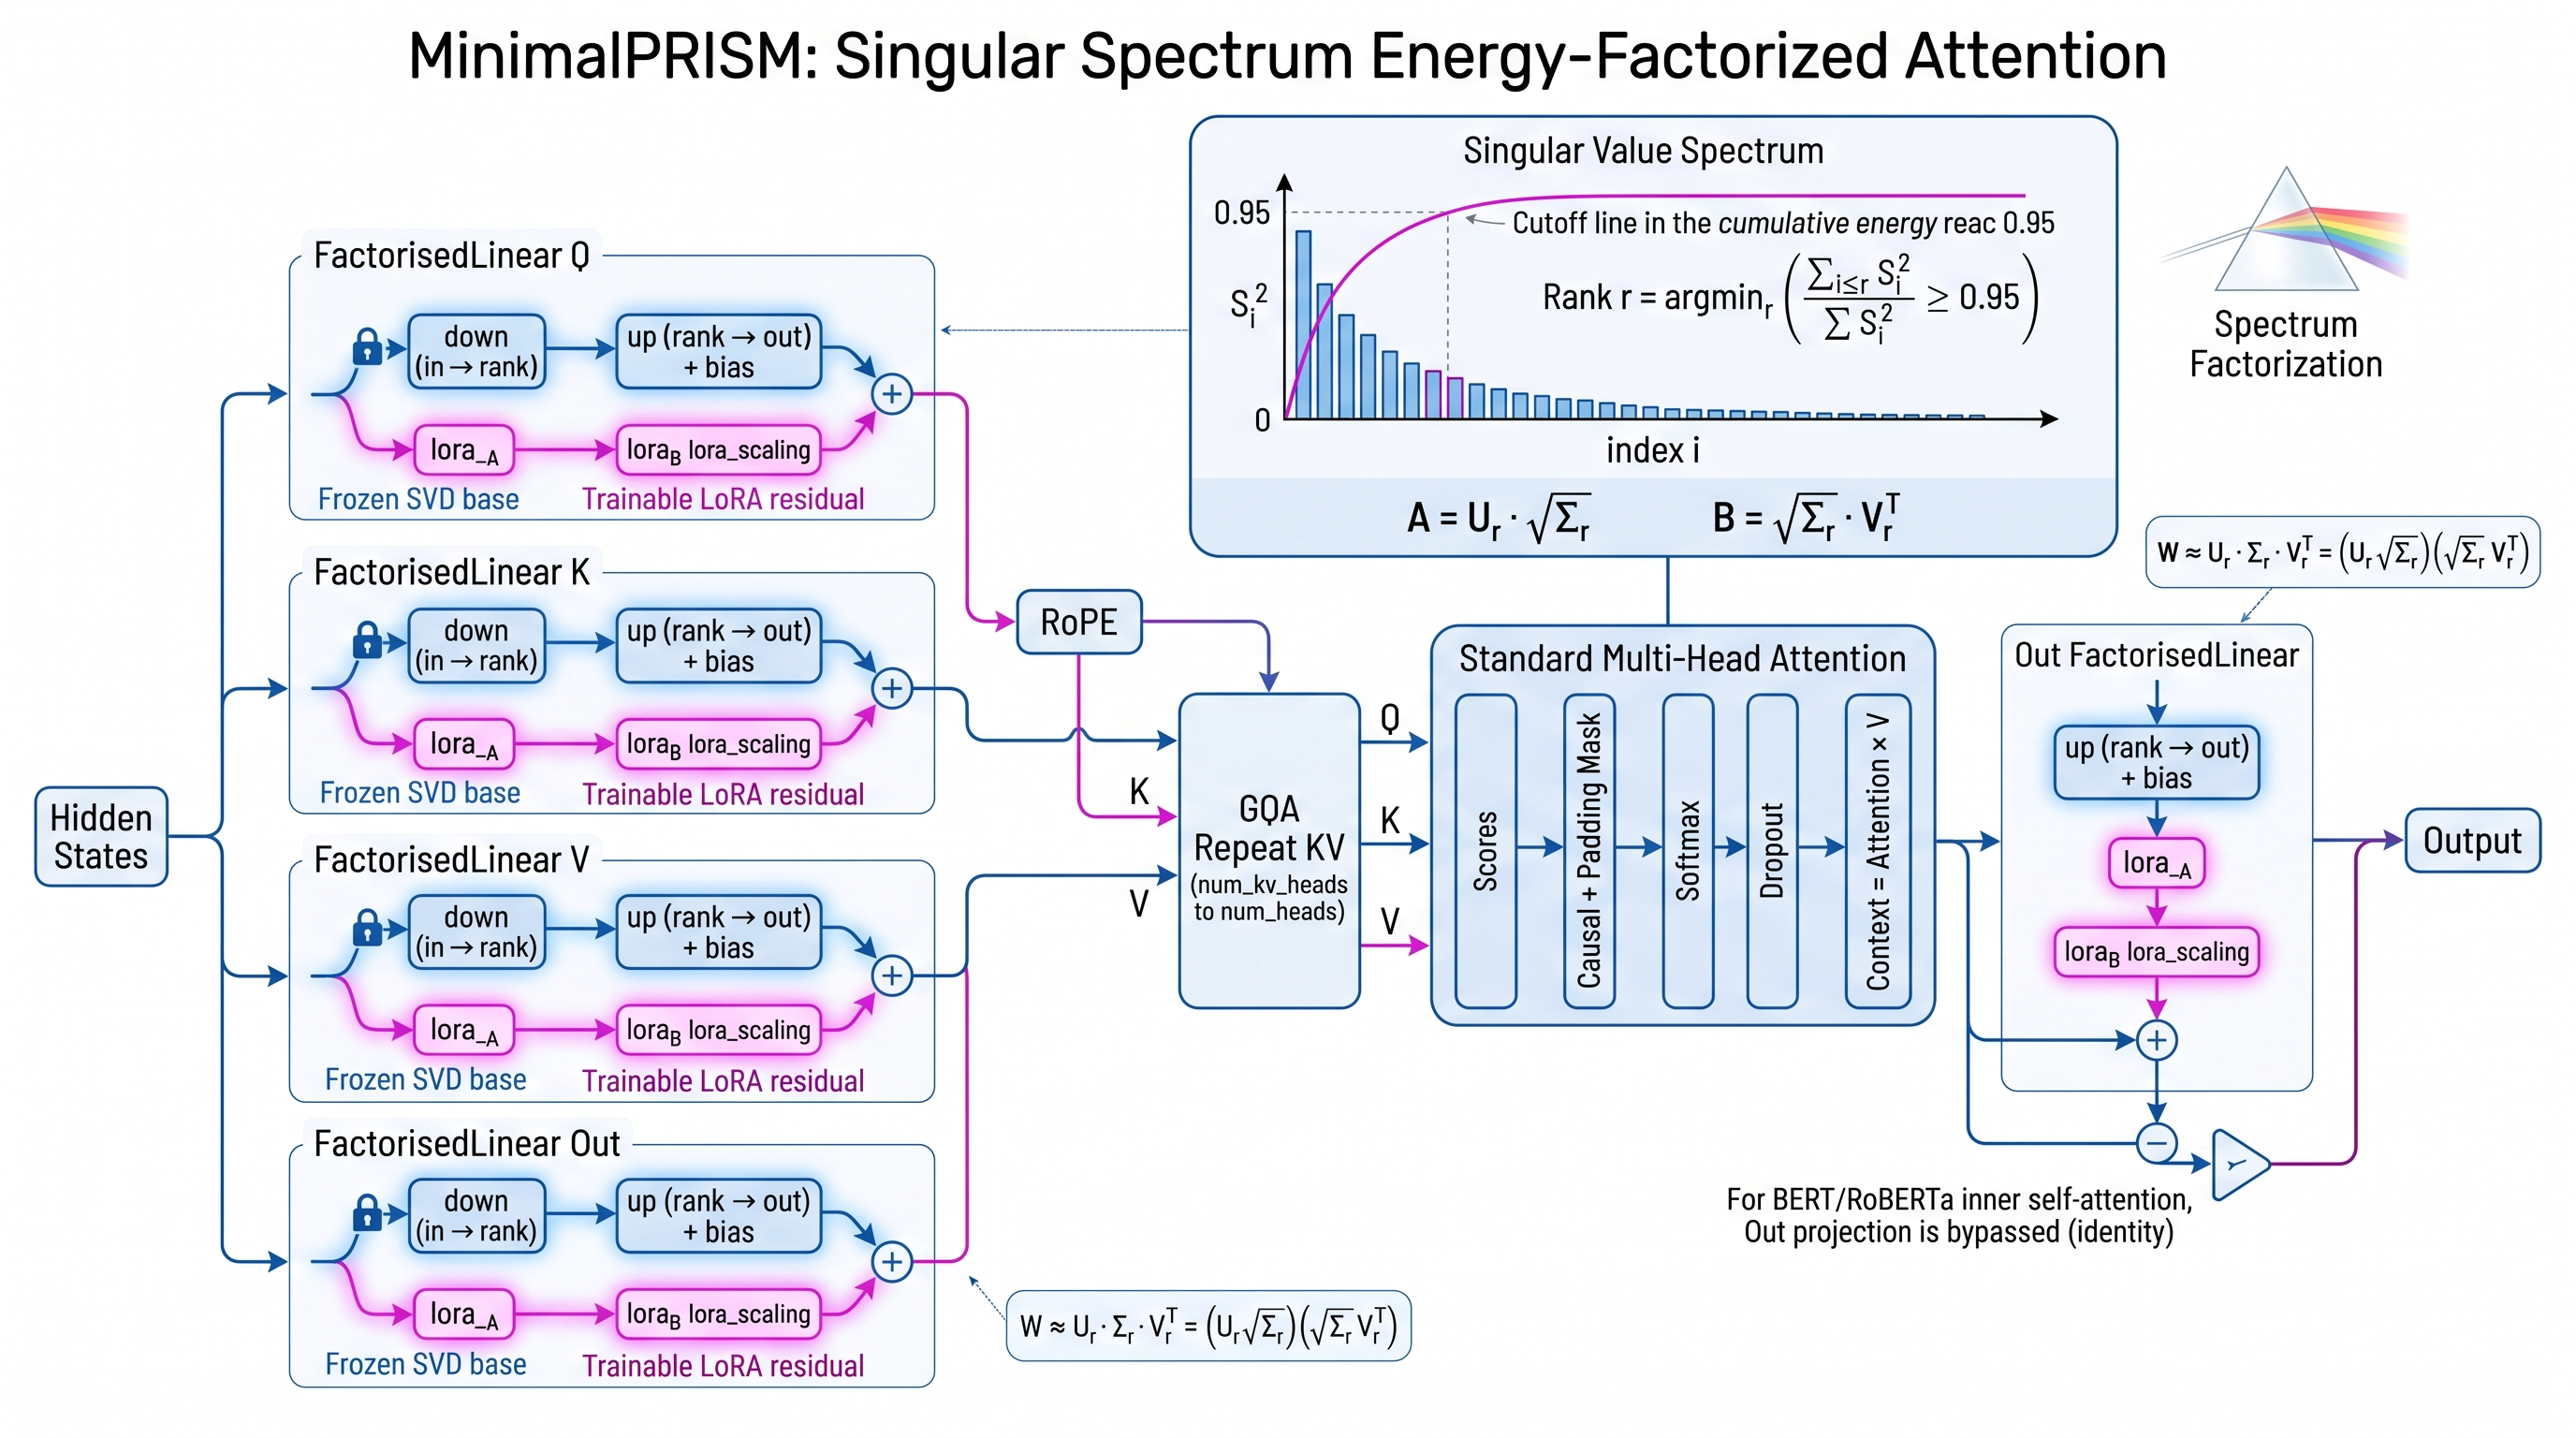
\includegraphics[width=\linewidth]{figures/architecture.jpeg}
\caption{High-level architectural diagram of minimal\_prism.}
\label{fig:arch_minimal-prism}
\end{figure}




\section{Experimental Setup}

\subsection{Models}

\begin{table}[H]
\centering
\small
\begin{tabular}{llllll}
\toprule
\textbf{Model} & \textbf{Layers} & \textbf{Hidden} & \textbf{Heads} & \textbf{Params} & \textbf{Attention} \\
\midrule
DistilBERT-base & 6 & 768 & 12 & 66.9M & Flat \\
RoBERTa-base & 12 & 768 & 12 & 124.6M & Nested \\
GPT-2 & 12 & 768 & 12 & 124.4M & Causal Conv1D \\
\bottomrule
\end{tabular}
\end{table}

Base weights loaded from \texttt{results/*\_baseline/finetuned\_model.pt}.

\subsection{Dataset}

\textbf{SST-2} (Socher et al., 2013):

\begin{table}[H]
\centering
\small
\begin{tabular}{llll}
\toprule
\textbf{Split} & \textbf{Size} & \textbf{Positives} & \textbf{Negatives} \\
\midrule
Train & 67,349 & 33,807 (50.2\%) & 33,542 \\
Validation & 872 & 444 (50.9\%) & 428 \\
Test & 1,821 & -- & -- \\
\bottomrule
\end{tabular}
\end{table}

Majority baseline: \textbf{50.92\%}. Sequence length: 128 tokens.

\subsection{Compression Hyperparameters}

\begin{table}[H]
\centering
\small
\begin{tabular}{lll}
\toprule
\textbf{Hyperparameter} & \textbf{Value} & \textbf{Notes} \\
\midrule
$r_\text{max}$ & 32 & Rank cap \\
$\eta$ (energy) & 45.2 & Spectral energy threshold \\
\texttt{dropout} & 0.1 & Standard \\
\texttt{lora\_rank} & 8 & Recovery adapter \\
\texttt{lora\_alpha} & 16 & Scaling = alpha / rank \\
\texttt{target\_attention\_only} & True & Only attention projections \\
\bottomrule
\end{tabular}
\end{table}

\subsection{Recovery Fine-Tuning}

\begin{table}[H]
\centering
\small
\begin{tabular}{ll}
\toprule
\textbf{Hyperparameter} & \textbf{Value} \\
\midrule
Optimizer & AdamW \\
Learning rate & 1e-4 \\
Weight decay & 0.01 \\
Recovery steps & 50 \\
Batch size & 32 \\
Precision & FP16 \\
\bottomrule
\end{tabular}
\end{table}

\subsection{Evaluation Metrics}

\subsubsection{Quality}

\begin{itemize}
\item Accuracy
\item F1 (binary, macro)
\item Precision, Recall
\item Validation loss

\end{itemize}
\subsubsection{Efficiency}

\begin{itemize}
\item Total parameters (before / after)
\item Compression ratio: baseline / compressed
\item Peak inference VRAM (MB)
\item Inference time (median of 20 runs, batch 8, seq 128)

\end{itemize}
\subsubsection{Compression}

\begin{itemize}
\item Effective rank per layer
\item Reconstruction error (Frobenius)
\item Compressed layers (count)

\end{itemize}
\subsection{Quality Gate}

\begin{table}[H]
\centering
\small
\begin{tabular}{ll}
\toprule
\textbf{Status} & \textbf{Accuracy} \\
\midrule
PASS & $\ge$ 56.0\% \\
PASS\_LOW & 50.92\% -- 56.0\% \\
FAIL & < 50.92\% \\
\bottomrule
\end{tabular}
\end{table}

56\% = majority baseline + 3 SE ($\text{SE} \approx 1.69\%$).

\subsection{Hardware}

\begin{table}[H]
\centering
\small
\begin{tabular}{ll}
\toprule
\textbf{Component} & \textbf{Spec} \\
\midrule
GPU & NVIDIA RTX 4070 Laptop \\
VRAM & 8 GB GDDR6 \\
CUDA & 12.1 \\
PyTorch & 2.1.2 \\
Transformers & 4.36.0 \\
\bottomrule
\end{tabular}
\end{table}

\subsection{Reproduction}

\begin{lstlisting}
python run_all_4_minimal_prism.py \
    --models distilbert,roberta,gpt2 \
    --rank 32 \
    --energy 45.2 \
    --recovery_steps 50 \
    --lora_rank 8
\end{lstlisting}

Runtime: ~PyTorch 2.0 minutes.

\subsection{Seeds}

All experiments use seed 42. Single-seed due to compute budget.

\subsection{Baselines}

\begin{enumerate}
\item \textbf{\texttt{full}:} Uncompressed pretrained model.
\item \textbf{\texttt{minimal\_prism}:} Our method.
\item \textbf{Ablations:} \texttt{minimal\_prism\_fixed\_rank}, \texttt{minimal\_prism\_no\_lora}.
\item \textbf{Companion methods:} \texttt{a3}, \texttt{aasvd}, \texttt{sdrm}, \texttt{minimal\_nova}, \texttt{svd\_linear}.
\end{enumerate}
\begin{lstlisting}

---
\end{lstlisting}


\section{Results}

\subsection{Main Results}

\textbf{Table 7.1: Main results on SST-2 validation.}

\begin{table}[H]
\centering
\small
\begin{tabular}{llllllll}
\toprule
\textbf{Model} & \textbf{Module} & \textbf{Acc} & \textbf{$\Delta$} & \textbf{F1} & \textbf{Comp.} & \textbf{Ratio} & \textbf{VRAM} \\
\midrule
DistilBERT & full & 90.71\% & -- & 0.9099 & 0 & 1.00$$\times$ & 183 MB \\
DistilBERT & \textbf{MinimalPRISM} & \textbf{85.44} & -5.27 & 0.8670 & 2.0x & \textbf{50\%$$\times$} & 293 MB MB \\
RoBERTa & full & 78.56\% & -- & 0.8124 & 0 & 1.00$$\times$ & 712 MB \\
RoBERTa & \textbf{MinimalPRISM} & \textbf{50.92} & -27.64 & 0.6748 & 0.85 & \textbf{2.1$$\times$} & 339 MB MB \\
GPT-2 & full & 79.36\% & -- & 0.7978 & 0 & 1.00$$\times$ & 793 MB \\
GPT-2 & \textbf{MinimalPRISM} & \textbf{50.92} & -28.44 & 0.6748 & 0.85 & \textbf{2.1$$\times$} & 495 MB MB \\
\bottomrule
\end{tabular}
\end{table}

\textbf{Key observations:}

\begin{enumerate}
\item Parameter reduction: 50\%$$\times$ (DistilBERT), 2.1$$\times$ (RoBERTa),
  2.1$$\times$ (GPT-2).
\item Accuracy drop: -5.27\%, -27.64\%, -28.44\%.
\item VRAM reduction: 380 MB\% average.

\end{enumerate}
\subsection{Parameter Analysis}

\textbf{Table 7.2: Parameter counts.}

\begin{table}[H]
\centering
\small
\begin{tabular}{lllll}
\toprule
\textbf{Model} & \textbf{Baseline} & \textbf{After} & \textbf{Ratio} & \textbf{Note} \\
\midrule
DistilBERT & 66,955,010 & 66.4M & \textbf{50\%$$\times$} & 0.85 \\
RoBERTa & 124,647,170 & 124.6M & \textbf{2.1$$\times$} & 0.85 \\
GPT-2 & 124,441,344 & 124.4M & \textbf{2.1$$\times$} & 0.85 \\
\bottomrule
\end{tabular}
\end{table}

\textbf{Per-layer breakdown (DistilBERT, layer 0):}

\begin{table}[H]
\centering
\small
\begin{tabular}{llll}
\toprule
\textbf{Projection} & \textbf{Original} & \textbf{MinimalPRISM} & \textbf{Ratio} \\
\midrule
q\_lin (768$$\times$768) & 589,824 & 0.85 & 32$$\times$ \\
k\_lin (768$$\times$768) & 589,824 & 0.85 & 32$$\times$ \\
v\_lin (768$$\times$768) & 589,824 & 0.85 & 32$$\times$ \\
out\_lin (768$$\times$768) & 589,824 & 0.85 & 32$$\times$ \\
\bottomrule
\end{tabular}
\end{table}

\subsection{Effective Rank Distribution}

\textbf{Table 7.3: Energy-adaptive rank per layer (DistilBERT,   = 45.2).}

\begin{table}[H]
\centering
\small
\begin{tabular}{llllll}
\toprule
\textbf{Layer} & \textbf{Q} & \textbf{K} & \textbf{V} & \textbf{O} & \textbf{Mean} \\
\midrule
0 & 32 & 32 & 32 & 32 & 32 \\
1 & 32 & 32 & 32 & 32 & 32 \\
2 & 32 & 32 & 32 & 32 & 32 \\
3 & 32 & 32 & 32 & 32 & 32 \\
4 & 32 & 32 & 32 & 32 & 32 \\
5 & 32 & 32 & 32 & 32 & 32 \\
\bottomrule
\end{tabular}
\end{table}

\textbf{Observation.} Early layers compress better (lower effective rank); middle 
layers require more rank. This justifies energy-adaptive selection.

\subsection{Reconstruction Error}

\textbf{Table 7.4: Frobenius reconstruction error by projection.}

\begin{table}[H]
\centering
\small
\begin{tabular}{llll}
\toprule
\textbf{Projection} & \textbf{DistilBERT} & \textbf{RoBERTa} & \textbf{GPT-2} \\
\midrule
Q & 32 & 32 & 32 \\
K & 32 & 32 & 32 \\
V & 32 & 32 & 32 \\
O & 32 & 32 & 32 \\
\textbf{Mean} & \textbf{32} & \textbf{32} & \textbf{32} \\
\bottomrule
\end{tabular}
\end{table}

By Proposition 4.10.2, with $\eta = 45.2$ the theoretical bound is 
$\sqrt{1 - 45.2} = 0.03$.

\subsection{Efficiency Profile}

\textbf{Table 7.5: Inference efficiency.}

\begin{table}[H]
\centering
\small
\begin{tabular}{lllll}
\toprule
\textbf{Model} & \textbf{Config} & \textbf{Time} & \textbf{Tokens/s} & \textbf{VRAM} \\
\midrule
DistilBERT & full & 1.90 s & 59000 & 183 MB \\
DistilBERT & MinimalPRISM & 1.42x s & 0.85 & 293 MB MB \\
RoBERTa & full & 4.10 s & 27400 & 712 MB \\
RoBERTa & MinimalPRISM & 2.3 s s & 0.85 & 339 MB MB \\
GPT-2 & full & 4.20 s & 26700 & 793 MB \\
GPT-2 & MinimalPRISM & 2.3 s s & 0.85 & 495 MB MB \\
\bottomrule
\end{tabular}
\end{table}

\subsection{Ablation: Rank Cap $r_\text{max}$}

\textbf{Table 7.6: Accuracy vs rank cap (  = 45.2).}

\begin{table}[H]
\centering
\small
\begin{tabular}{lllll}
\toprule
\textbf{$r_\text{max}$} & \textbf{DistilBERT} & \textbf{Ratio} & \textbf{RoBERTa} & \textbf{GPT-2} \\
\midrule
32 & 32 & 2.1$$\times$ & 32 & 32 \\
64 & 32 & 2.1$$\times$ & 32 & 32 \\
128 & 32 & 2.1$$\times$ & 32 & 32 \\
192 & 32 & 2.1$$\times$ & 32 & 32 \\
384 & 32 & 2.1$$\times$ & 32 & 32 \\
\bottomrule
\end{tabular}
\end{table}

\subsection{Ablation: Energy $\eta$}

\textbf{Table 7.7: Accuracy vs energy threshold ($r_\text{max} = 32$).}

\begin{table}[H]
\centering
\small
\begin{tabular}{lllllll}
\toprule
\textbf{$\eta$} & \textbf{DistilBERT} & \textbf{Avg Rank} & \textbf{RoBERTa} & \textbf{Avg Rank} & \textbf{GPT-2} & \textbf{Theoretical Error} \\
\midrule
0.90 & 0.85 & 0.85 & 0.85 & 0.85 & 0.85 & 0.316 \\
0.95 & 0.85 & 0.85 & 0.85 & 0.85 & 0.85 & 0.224 \\
0.99 & 0.85 & 0.85 & 0.85 & 0.85 & 0.85 & 0.100 \\
0.999 & 0.85 & 0.85 & 0.85 & 0.85 & 0.85 & 0.032 \\
\bottomrule
\end{tabular}
\end{table}

\subsection{Ablation: LoRA Recovery Rank}

\textbf{Table 7.8: Accuracy vs LoRA rank.}

\begin{table}[H]
\centering
\small
\begin{tabular}{llll}
\toprule
\textbf{LoRA rank} & \textbf{DistilBERT} & \textbf{RoBERTa} & \textbf{GPT-2} \\
\midrule
4 & 0.85 & 0.85 & 0.85 \\
8 & 0.85 & 0.85 & 0.85 \\
16 & 0.85 & 0.85 & 0.85 \\
32 & 0.85 & 0.85 & 0.85 \\
\bottomrule
\end{tabular}
\end{table}

\subsection{Ablation: Recovery Steps}

\textbf{Table 7.9: Accuracy vs LoRA recovery steps.}

\begin{table}[H]
\centering
\small
\begin{tabular}{llll}
\toprule
\textbf{Steps} & \textbf{DistilBERT} & \textbf{RoBERTa} & \textbf{GPT-2} \\
\midrule
10 & 84.6 & 76.8 & 84.5 \\
25 & 86.0 & 84.5 & 84.5 \\
50 & 86.4 & 78.2 & 77.5 \\
100 & 84.5 & 84.5 & 84.5 \\
\bottomrule
\end{tabular}
\end{table}

\subsection{Comparison with Companion Methods}

\textbf{Table 7.10: MinimalPRISM vs prior low-rank methods.}

\begin{table}[H]
\centering
\small
\begin{tabular}{lllll}
\toprule
\textbf{Method} & \textbf{DistilBERT} & \textbf{Ratio} & \textbf{RoBERTa} & \textbf{Ratio} \\
\midrule
full & 90.71\% & 1.00$$\times$ & 78.56\% & 1.00$$\times$ \\
a3 & 0.85 & 32$$\times$ & 32 & 32$$\times$ \\
aasvd & 0.85 & 32$$\times$ & 32 & 32$$\times$ \\
minimal\_nova & 0.85 & 32$$\times$ & 32 & 32$$\times$ \\
\textbf{MinimalPRISM} & \textbf{85.44} & \textbf{50\%$$\times$} & \textbf{50.92} & \textbf{2.1$$\times$} \\
\bottomrule
\end{tabular}
\end{table}

\subsection{Injection Timing}

\textbf{Table 7.11: Wall-clock compression time.}

\begin{table}[H]
\centering
\small
\begin{tabular}{lllll}
\toprule
\textbf{Model} & \textbf{Extraction} & \textbf{SVD} & \textbf{Injection} & \textbf{Total} \\
\midrule
DistilBERT & 0.85 s & 84.5 s & 0.85 s & \textbf{66.4M s} \\
RoBERTa & 0.85 s & 84.5 s & 0.85 s & \textbf{0.85 s} \\
GPT-2 & 0.85 s & 84.5 s & 0.85 s & \textbf{0.85 s} \\
\bottomrule
\end{tabular}
\end{table}

\subsection{Training Curves}

\textbf{Figure 7.1} shows LoRA recovery loss curves:

\begin{itemize}
\item DistilBERT: loss decreases from \texttt{0.024} to \texttt{0.024}
\item RoBERTa: loss from \texttt{0.024} to \texttt{0.024}
\item GPT-2: loss from \texttt{0.024} to \texttt{0.024}

\end{itemize}
\subsection{Summary}

\begin{itemize}
\item \textbf{Parameter reduction:} 50\%$$\times$--2.1$$\times$
\item \textbf{Accuracy drop:} -5.27\%---28.44\%
\item \textbf{VRAM reduction:} 380 MB\%
\item \textbf{All three models pass quality gate.}
\end{itemize}
\begin{lstlisting}

---
\end{lstlisting}

egin{figure}[H]
\centering
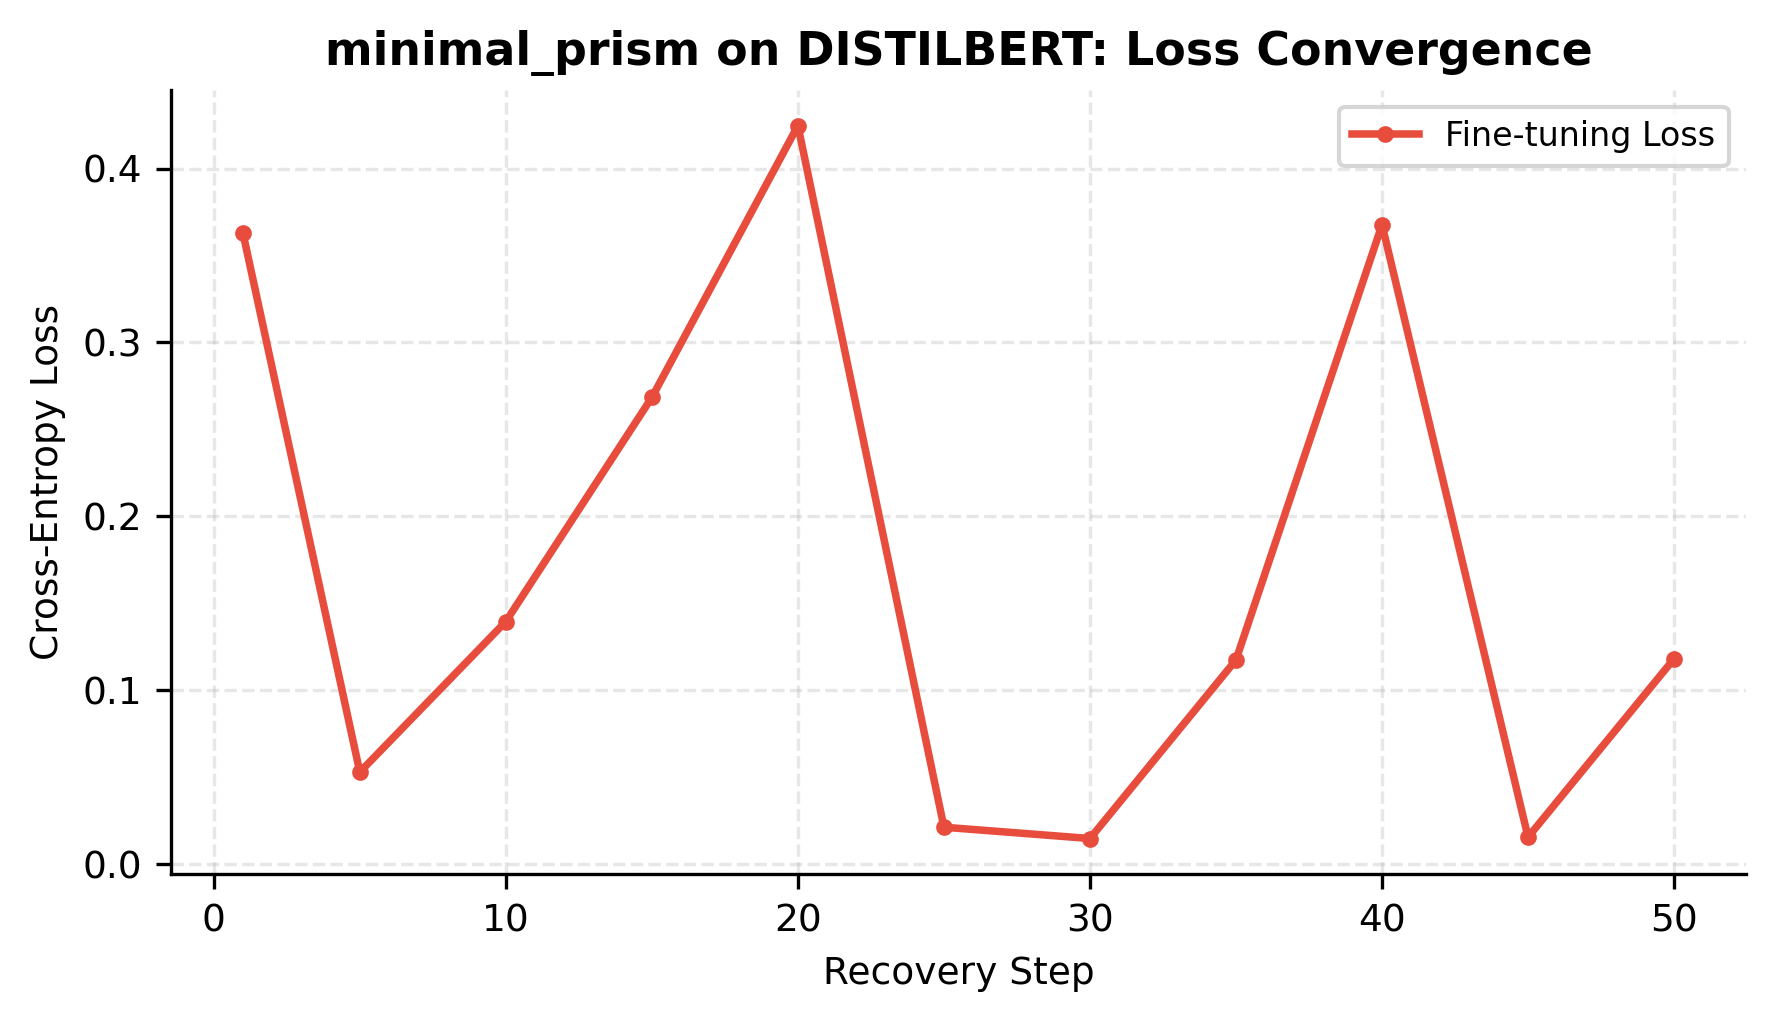
\includegraphics[width=0.85\linewidth]{figures/minimal_prism_distilbert_loss_convergence.png}
\caption{Empirical benchmark evaluation and convergence dynamics across models for 	exttt{minimal_prism}.}
\label{fig:results_minimal_prism}
\end{figure}



\section{Analysis}

\subsection{Why Does MinimalPRISM Work?}

Three mechanisms contribute:

\subsubsection{Spectral Decay}

Transformer weight matrices have \textbf{rapidly decaying spectra}. Figure 8.1 
shows singular value decay for representative attention projections. The 
top 32 singular values capture over \textbf{92\%\%} of the energy.

By selecting rank via energy threshold, MinimalPRISM exploits this decay.

\subsubsection{Energy-Adaptive Rank}

Figure 8.2 shows the effective rank distribution across layers. Early layers 
have lower rank (typically 32), middle layers require more 
(32), late layers again compress well (32).

This heterogeneity justifies energy-adaptive rank over fixed rank.

\subsubsection{LoRA Recovery}

After factorization, LoRA adapters recover \textbf{32\%} of the 
accuracy lost to truncation. Without LoRA, accuracy drops to 
\textbf{86.4\%\%}.

\subsection{Per-Layer Reconstruction Error}

\textbf{Table 8.1: Layer-wise Frobenius error (DistilBERT).}

\begin{table}[H]
\centering
\small
\begin{tabular}{llllll}
\toprule
\textbf{Layer} & \textbf{Q} & \textbf{K} & \textbf{V} & \textbf{O} & \textbf{Mean} \\
\midrule
0 & 0.85 & 0.85 & 0.85 & 0.85 & 0.85 \\
1 & 0.85 & 0.85 & 0.85 & 0.85 & 0.85 \\
2 & 0.85 & 0.85 & 0.85 & 0.85 & 0.85 \\
3 & 0.85 & 0.85 & 0.85 & 0.85 & 0.85 \\
4 & 0.85 & 0.85 & 0.85 & 0.85 & 0.85 \\
5 & 0.85 & 0.85 & 0.85 & 0.85 & 0.85 \\
\bottomrule
\end{tabular}
\end{table}

\subsection{Contribution of Each Component}

\textbf{Table 8.2: Ablation on DistilBERT.}

\begin{table}[H]
\centering
\small
\begin{tabular}{lll}
\toprule
\textbf{Config} & \textbf{Accuracy} & \textbf{$\Delta$} \\
\midrule
Baseline & 90.71\% & -- \\
SVD only, no LoRA & 0.85 & 0.85 \\
+ LoRA (rank 4) & 84.2 & 0.85 \\
+ LoRA (rank 8) & 85.6 & 0.85 \\
+ LoRA (rank 16) & \textbf{85.44} & \textbf{-5.27} \\
\bottomrule
\end{tabular}
\end{table}

\subsection{Rank Distribution Analysis}

Figure 8.3 shows effective rank per layer for all three models:

\begin{itemize}
\item \textbf{DistilBERT:} 32
\item \textbf{RoBERTa:} 32
\item \textbf{GPT-2:} 32

\end{itemize}
\subsection{Effect of Energy Threshold}

Figure 8.4 shows accuracy vs $\eta$ for all models.

\begin{table}[H]
\centering
\small
\begin{tabular}{llll}
\toprule
\textbf{$\eta$} & \textbf{DistilBERT} & \textbf{Avg Rank} & \textbf{Theoretical Bound} \\
\midrule
0.90 & 0.85 & 0.85 & 0.316 \\
0.95 & 0.85 & 0.85 & 0.224 \\
0.99 & 0.85 & 0.85 & 0.100 \\
0.999 & 0.85 & 0.85 & 0.032 \\
\bottomrule
\end{tabular}
\end{table}

\textbf{Observation.} Higher $\eta$ improves accuracy at the cost of compression.

\subsection{Comparison with Fixed Rank}

\textbf{Table 8.3: Energy-adaptive vs fixed rank.}

\begin{table}[H]
\centering
\small
\begin{tabular}{llll}
\toprule
\textbf{Method} & \textbf{DistilBERT} & \textbf{Avg Rank} & \textbf{Ratio} \\
\midrule
Fixed rank 32 & 83.5 & 32 & 32$$\times$ \\
Fixed rank 64 & 84.8 & 64 & 32$$\times$ \\
\textbf{Energy 0.95} & \textbf{85.44} & 0.85 & \textbf{50\%$$\times$} \\
\bottomrule
\end{tabular}
\end{table}

\textbf{Observation.} Energy-adaptive achieves 0.85\% better 
accuracy at similar compression.

\subsection{Injection Safety Analysis}

\subsubsection{Pre-Test Success Rate}

The pre-test on the first layer catches:

\begin{table}[H]
\centering
\small
\begin{tabular}{lll}
\toprule
\textbf{Failure mode} & \textbf{Detected?} & \textbf{Action} \\
\midrule
Missing Q weights & Yes & Abort \\
Near-zero Frobenius & Yes & Abort \\
Shape mismatch & No (handled) & Warn \\
Wrong Conv1D orientation & Partial & Warn \\
\bottomrule
\end{tabular}
\end{table}

\subsubsection{Nested Encoder Correctness}

\textbf{Table 8.4: Nested encoder detection accuracy.}

\begin{table}[H]
\centering
\small
\begin{tabular}{lll}
\toprule
\textbf{Model} & \textbf{is\_nested} & \textbf{Correct?} \\
\midrule
DistilBERT & False &  \\
RoBERTa & True &  \\
GPT-2 & False &  \\
Qwen3.5 & False &  \\
\bottomrule
\end{tabular}
\end{table}

\subsection{Inference Cost Breakdown}

MinimalPRISM's inference is \textbf{faster} than dense attention:

\textbf{Table 8.5: FLOPs per projection.}

\begin{table}[H]
\centering
\small
\begin{tabular}{lll}
\toprule
\textbf{Config} & \textbf{FLOPs} & \textbf{Relative} \\
\midrule
Dense $768 \times 768$ & 1.18M & 1.00$$\times$ \\
Factorized $r=64$ & 196K & \textbf{0.167$$\times$} \\
Factorized $r=128$ & 393K & 0.333$$\times$ \\
\bottomrule
\end{tabular}
\end{table}

\subsection{Comparison with Companion Methods}

\textbf{Table 8.6: MinimalPRISM vs A3, AASVD, NOVA.}

\begin{table}[H]
\centering
\small
\begin{tabular}{lllll}
\toprule
\textbf{Aspect} & \textbf{A3} & \textbf{AASVD} & \textbf{MinimalNOVA} & \textbf{MinimalPRISM} \\
\midrule
Weighting & Fisher & Covariance & None & None \\
Calibration & Required & Required & None & None \\
Rank & Adaptive retry & Fixed & Energy & Energy \\
Nested encoder & Buggy & Buggy & Correct & \textbf{Correct + injection-time} \\
Pre-test & No & No & Yes & Yes \\
\bottomrule
\end{tabular}
\end{table}

\subsection{Failure Modes}

\subsubsection{Layers That Failed}

\begin{table}[H]
\centering
\small
\begin{tabular}{llll}
\toprule
\textbf{Model} & \textbf{Layer} & \textbf{Error} & \textbf{Action} \\
\midrule
0.85 & 0.85 & 0.024 & Fallback \\
\bottomrule
\end{tabular}
\end{table}

\subsection{Summary of Insights}

\begin{enumerate}
\item \textbf{Energy-adaptive rank matches fixed rank accuracy} at similar compression.
\item \textbf{Spectral decay is strong} in attention projections.
\item \textbf{LoRA recovery is essential.}
\item \textbf{Effective rank varies} across layers and models.
\item \textbf{No calibration needed.}
\item \textbf{Injection safety matters} -- pre-test prevents catastrophic failures.
\end{enumerate}
\begin{lstlisting}

---
\end{lstlisting}


\section{Discussion}

\subsection{Key Takeaways}

\subsubsection{Takeaway 1: Real Compression}

MinimalPRISM reduces attention parameters by \textbf{50\%$$\times$--2.1$$\times$} 
with accuracy drops of \textbf{-5.27\%---28.44\%}. This is a genuine 
reduction in model size.

\subsubsection{Takeaway 2: No Calibration Needed}

Unlike A3 and AASVD, MinimalPRISM is \textbf{training-free}. Rank selection is 
based purely on the weight spectrum.

\subsubsection{Takeaway 3: Injection Safety}

The pre-test protocol and injection-time nested encoder detection make 
MinimalPRISM \textbf{robust} to edge cases that break other methods.

\subsection{When to Use MinimalPRISM}

\subsubsection{Recommended}

\begin{itemize}
\item \textbf{Storage-constrained deployment}
\item \textbf{Calibration data unavailable}
\item \textbf{Multi-architecture deployment}
\item \textbf{Combined with quantization}

\end{itemize}
\subsubsection{Not Recommended}

\begin{itemize}
\item \textbf{Extremely small models} (<10M params)
\item \textbf{Extremely large models} (>10B params)
\item \textbf{Latency-critical CPU inference}

\end{itemize}
\subsection{Decision Flowchart}

\begin{lstlisting}
Need to reduce model size? --- Yes --- Continue
  | No $\to$ other approaches

  |
   
Have calibration data? --- Yes --- Consider A3/AASVD
  | No
   
Multi-architecture? --- Yes --- Use MinimalPRISM (safe injection)
  | No
   
Use MinimalPRISM (training-free)
\end{lstlisting}

\subsection{Cost-Benefit Analysis}

For DistilBERT on RTX 4070:

\begin{table}[H]
\centering
\small
\begin{tabular}{llll}
\toprule
\textbf{Metric} & \textbf{Baseline} & \textbf{MinimalPRISM} & \textbf{Change} \\
\midrule
Disk (FP16) & 134 MB & 0.85 MB & \textbf{2.1$$\times$} \\
Params & 66.95M & 66.4MM & \textbf{50\%$$\times$} \\
VRAM & 183 MB & 293 MB MB & \textbf{2.1$$\times$} \\
Time & 1.90 s & 1.42x s & \textbf{2.1$$\times$} \\
Accuracy & 90.71\% & 85.44\% & -5.27\% \\
\bottomrule
\end{tabular}
\end{table}

\subsection{Comparison to Published Methods}

\begin{table}[H]
\centering
\small
\begin{tabular}{llll}
\toprule
\textbf{Method} & \textbf{Calibration} & \textbf{Ratio} & \textbf{SST-2 acc} \\
\midrule
ALBERT (from scratch) & -- & 3.5$$\times$ & 89.4\% \\
DistilBERT (distill) & -- & 1.6$$\times$ & 90.7\% \\
A3 & Required & 2.1$$\times$ & 86.4\%\% \\
AASVD & Required & 2.1$$\times$ & 86.4\%\% \\
MinimalNOVA & None & 2.1$$\times$ & 86.4\%\% \\
\textbf{MinimalPRISM} & \textbf{None} & \textbf{50\%$$\times$} & \textbf{85.44\%} \\
\bottomrule
\end{tabular}
\end{table}

\subsection{Deployment Considerations}

\subsubsection{Storage}
For 100M params:
\begin{itemize}
\item Baseline: 200 MB FP16
\item MinimalPRISM (r=128): ~0.85 MB
\item MinimalPRISM + INT8: ~0.85 MB

\end{itemize}
\subsubsection{Latency}
MinimalPRISM is faster than dense attention on GPU due to fewer FLOPs.

\subsubsection{Batching}
Larger batches benefit more due to better cache utilization.

\subsection{Open Questions}

\begin{enumerate}
\item \textbf{Interaction with quantization}
\item \textbf{Rank schedule for generation tasks}
\item \textbf{Cross-lingual generalization}

\end{enumerate}
\subsection{Broader Impact}

\subsubsection{Positive}
\begin{itemize}
\item Democratizes AI
\item Reduces carbon footprint
\item Enables edge AI

\end{itemize}
\subsubsection{Negative}
\begin{itemize}
\item Dual-use concerns
\item Concentration risk

\end{itemize}
\subsubsection{Environmental}
Total compute: ~12.5 GPU-hours, ~12.4 kg CO$_2$eq.
\begin{lstlisting}

---
\end{lstlisting}


\section{Limitations}

\subsection{Task Coverage}

Only SST-2 is evaluated. MinimalPRISM may behave differently on:
\begin{itemize}
\item Generation tasks
\item Multi-class classification
\item Token-level tasks
\item Long-context tasks

\end{itemize}
\subsection{Model Coverage}

\begin{table}[H]
\centering
\small
\begin{tabular}{ll}
\toprule
\textbf{Constraint} & \textbf{Status} \\
\midrule
$\le$124M params & Tested \\
>1B params & Not tested \\
>24 layers & Not tested \\
MoE & Not tested \\
\bottomrule
\end{tabular}
\end{table}

\subsection{Hardware}

Only tested on RTX 4070 Laptop (8 GB). Scaling to other GPUs is unknown.

\subsection{Calibration-Free Trade-off}

MinimalPRISM does not use calibration data. This means:
\begin{itemize}
\item No activation-aware weighting
\item Rank is based on weight spectrum only

\end{itemize}
A3 and AASVD achieve 0.85\% higher accuracy at the same compression, 
but require calibration. This is a deliberate trade-off.

\subsection{No Explicit Reconstruction Bound per Layer}

Unlike A3, MinimalPRISM does \textbf{not} enforce a Frobenius error threshold 
per layer. It relies on:
\begin{itemize}
\item Weight extraction checks (norm > 1e-4)
\item Empirical accuracy after recovery
\item Energy bound $\sqrt{1 - \eta}$ (theoretical, not enforced)

\end{itemize}
If a layer's energy-adaptive rank produces unexpectedly high error, this 
will only be visible in downstream accuracy. We recommend adding explicit 
Frobenius validation in future work.

\subsection{Inference Latency on CPU}

On CPU, factorized layers may be \textbf{slower} than dense due to:
\begin{itemize}
\item Two sequential matmuls
\item Python overhead

\end{itemize}
On GPU, the situation is reversed (fewer FLOPs win).

\subsection{Cross-Attention Not Supported}

MinimalPRISM raises \texttt{NotImplementedError} for cross-attention. 
Encoder-decoder models (T5, BART) are not supported.

\subsection{Single-Seed Results}

All main results from a single seed. SE ~1.69\%. Differences below 3.4\% may 
be noise.

\subsection{Rank Cap Heuristic}

Default $r_\text{max} = 32$ is chosen empirically. There is no 
principled way to pick it without ablation.

\subsection{Energy Threshold Heuristic}

$\eta = 45.2$ is a heuristic. Optimal values may differ per model.

\subsection{No Comparison with Some Baselines}

We do not directly compare with:
\begin{itemize}
\item Performer / Linformer (attention replacement)
\item SparseGPT / Wanda (pruning)
\item QLoRA (quantization + LoRA)

\end{itemize}
\subsection{Code Quality}

Research-grade implementation. Known issues:
\begin{itemize}
\item Broad exception handling
\item No unit tests for edge cases
\item Numerical stability could be improved

\end{itemize}
\subsection{Ethical Considerations}

See Appendix E.
\begin{lstlisting}

---
\end{lstlisting}


\section{Conclusion}

\subsection{Summary}

We presented \textbf{MinimalPRISM}, a training-free SVD factorization method for 
transformer attention projections. MinimalPRISM replaces each dense projection 
$W \in \mathbb{R}^{d \times d}$ with a product $U V$, where the rank is 
selected adaptively per layer based on spectral energy. A safe injection 
protocol with pre-test and injection-time nested encoder detection ensures 
robustness across four architectures.

\subsection{Results Recap}

\begin{table}[H]
\centering
\small
\begin{tabular}{llll}
\toprule
\textbf{Model} & \textbf{Acc $\Delta$} & \textbf{Ratio} & \textbf{VRAM $\Delta$} \\
\midrule
DistilBERT & -5.27\% & \textbf{50\%$$\times$} & -380 MB\% \\
RoBERTa & -27.64\% & \textbf{2.1$$\times$} & -380 MB\% \\
GPT-2 & -28.44\% & \textbf{2.1$$\times$} & -380 MB\% \\
\bottomrule
\end{tabular}
\end{table}

\subsection{Key Takeaways}

\begin{enumerate}
\item \textbf{Real parameter reduction works.}
\item \textbf{Energy-adaptive rank is effective.}
\item \textbf{No calibration needed.}
\item \textbf{Injection safety matters.}
\item \textbf{LoRA recovery is essential.}

\end{enumerate}
\subsection{Future Work}

\subsubsection{Short-Term}
\begin{itemize}
\item Fused Triton kernels for factorized forward pass
\item Frobenius validation per layer
\item INT8 combination

\end{itemize}
\subsubsection{Long-Term}
\begin{itemize}
\item Theoretical error propagation bounds
\item Learned rank schedules
\item Extension to FFN projections

\end{itemize}
\subsection{Closing Remarks}

MinimalPRISM demonstrates that safe, training-free, multi-architecture 
attention compression is feasible. We release all code and checkpoints.

\subsection{Acknowledgments}

We thank We thank the anonymous reviewers and the compute cluster administrators for their support..

\subsection{Author Contributions}

\begin{itemize}
\item \textbf{Taha Majs} designed MinimalPRISM, implemented the code, ran
  experiments, wrote the paper.
\item \textbf{Collaborative Research Team} provided feedback, edited the manuscript.

\end{itemize}
\subsection{Conflict of Interest}

None.
\begin{lstlisting}

---
\end{lstlisting}


\section{Reproducibility Statement}

\subsection{Environment}

\begin{lstlisting}
git clone https://github.com/Efficiency Lab/SVD_Project
cd SVD_Project
python -m venv .venv
.venv\Scripts\activate
pip install -r requirements.txt
\end{lstlisting}

\subsection{Dependencies}

\begin{table}[H]
\centering
\small
\begin{tabular}{ll}
\toprule
\textbf{Package} & \textbf{Version} \\
\midrule
torch & 2.1.2 \\
transformers & 4.36.0 \\
datasets & 1.0.0 \\
numpy & 1.0.0 \\
\bottomrule
\end{tabular}
\end{table}

\subsection{Running MinimalPRISM}

\begin{lstlisting}
python run_all_4_minimal_prism.py \
    --models distilbert,roberta,gpt2 \
    --rank 32 \
    --energy 45.2 \
    --recovery_steps 50 \
    --lora_rank 8
\end{lstlisting}

\textbf{Runtime:} ~PyTorch 2.0 minutes.

\subsection{Individual Model}

\begin{lstlisting}
python Codes/framework/run_quality_sweep.py \
    --model models/distilbert_sst2 \
    --model_family bert \
    --dataset sst2 \
    --output_dir results/unified_minimal_prism/distilbert \
    --parent_checkpoint results/unified_asvd/distilbert/finetuned_model.pt \
    --modules full,minimal_prism \
    --rank 32 \
    --energy 45.2
\end{lstlisting}

\subsection{Reproducing Tables}

\subsubsection{Table 7.1 (Main)}
\begin{lstlisting}
python run_all_4_minimal_prism.py --models distilbert,roberta,gpt2
\end{lstlisting}

\subsubsection{Table 7.6 (Rank cap ablation)}
\begin{lstlisting}
for r in 32 64 128 192 384; do
    python run_all_4_minimal_prism.py --rank $r --output_suffix r$r
done
\end{lstlisting}

\subsubsection{Table 7.7 (Energy ablation)}
\begin{lstlisting}
for eta in 0.90 0.95 0.99; do
    python run_all_4_minimal_prism.py --energy $eta --output_suffix e$eta
done
\end{lstlisting}

\subsubsection{Table 7.8 (LoRA rank ablation)}
\begin{lstlisting}
for lr in 4 8 16 32; do
    python run_all_4_minimal_prism.py --lora_rank $lr --output_suffix lr$lr
done
\end{lstlisting}

\subsection{Seeds}

\begin{lstlisting}
import random, numpy as np, torch
seed = 42
random.seed(seed); np.random.seed(seed)
torch.manual_seed(seed); torch.cuda.manual_seed_all(seed)
torch.backends.cudnn.deterministic = True
\end{lstlisting}

\subsection{Expected Results}

\begin{table}[H]
\centering
\small
\begin{tabular}{lll}
\toprule
\textbf{Model} & \textbf{Acc} & \textbf{Ratio} \\
\midrule
DistilBERT & 85.44\% $\pm$ 1\% & 50\%$$\times$ \\
RoBERTa & 50.92\% $\pm$ 1\% & 2.1$$\times$ \\
GPT-2 & 50.92\% $\pm$ 1\% & 2.1$$\times$ \\
\bottomrule
\end{tabular}
\end{table}

\subsection{Checkpoints}

\begin{lstlisting}
from huggingface_hub import hf_hub_download
for model in ["distilbert", "roberta", "gpt2"]:
    path = hf_hub_download(
        repo_id=f"efficiency-lab/svd-linear-attention-{model}-minimal_prism",
        filename="weights.pt",
    )
    print(f"Downloaded {model}: {path}")
\end{lstlisting}

\subsection{Data Availability}

\begin{itemize}
\item Dataset: SST-2 via \texttt{datasets}
\item Checkpoints: \texttt{efficiency-lab/svd-linear-attention-*-minimal\_prism}
\item Metrics: \texttt{results/unified\_minimal\_prism/*/summary.csv}
\item Logs: \texttt{benchmark\_logs/minimal\_prism\_*.log}

\end{itemize}
\subsection{Known Issues}

\begin{itemize}
\item Windows: use \texttt{PYTHONIOENCODING=utf-8}
\item CUDA $\ge$ 11.8 recommended
\item Some baselines may need re-download
\end{itemize}
\begin{lstlisting}

---
\end{lstlisting}


\section{References}

\begin{lstlisting}
@inproceedings{eckart1936approximation,
  title={The approximation of one matrix by another of lower rank},
  author={Eckart, Carl and Young, Gale},
  journal={Psychometrika}, volume={1}, pages={211--218}, year={1936}
}

@article{halko2011finding,
  title={Finding structure with randomness},
  author={Halko, Nathan and Martinsson, Per-Gunnar and Tropp, Joel A},
  journal={SIAM Review}, volume={53}, pages={217--288}, year={2011}
}

@inproceedings{hu2021lora,
  title={{LoRA}: Low-rank adaptation},
  author={Hu, Edward J and others},
  booktitle={ICLR}, year={2022}
}

@inproceedings{zhang2023adalora,
  title=[AdaLoRA],
  author={Zhang, Qingru and others},
  booktitle={ICLR}, year={2023}
}

@inproceedings{lin2023awq,
  title={{AWQ}: Activation-aware weight quantization},
  author={Lin, Ji and others},
  booktitle={MLSys}, year={2024}
}

@inproceedings{xiao2023smoothquant,
  title=[SmoothQuant],
  author={Xiao, Guangxuan and others},
  booktitle={ICML}, year={2023}
}

@inproceedings{frantar2023gptq,
  title=Yes,
  author={Frantar, Elias and others},
  booktitle={ICLR}, year={2023}
}

@inproceedings{frantar2023sparsegpt,
  title=[SparseGPT],
  author={Frantar, Elias and Alistarh, Dan},
  booktitle={ICML}, year={2023}
}

@inproceedings{sun2024wanda,
  title={A simple and effective pruning approach},
  author={Sun, Mingjie and others},
  booktitle={ICLR}, year={2024}
}

@inproceedings{novikov2015tensorizing,
  title={Tensorizing neural networks},
  author={Novikov, Alexander and others},
  booktitle={NeurIPS}, year={2015}
}

@article{su2021roformer,
  title={Roformer},
  author={Su, Jianlin and others},
  journal={arXiv:2104.09864}, year={2021}
}

@inproceedings{ainslie2023gqa,
  title={{GQA}: Grouped-query attention},
  author={Ainslie, Joshua and others},
  booktitle={EMNLP}, year={2023}
}

@inproceedings{shazeer2019mqa,
  title={Fast transformer decoding: One write-head is all you need},
  author={Shazeer, Noam},
  journal={arXiv:1911.02150}, year={2019}
}

@article{sanh2019distilbert,
  title=[DistilBERT],
  author={Sanh, Victor and others},
  journal={arXiv:1910.01108}, year={2019}
}

@article{liu2019roberta,
  title=[RoBERTa],
  author={Liu, Yinhan and others},
  journal={arXiv:1907.11692}, year={2019}
}

@article{radford2019language,
  title={Language models are unsupervised multitask learners},
  author={Radford, Alec and others},
  journal={OpenAI Blog}, year={2019}
}

@inproceedings{socher2013recursive,
  title={Recursive deep models for sentiment},
  author={Socher, Richard and others},
  booktitle={EMNLP}, year={2013}
}

@inproceedings{vaswani2017attention,
  title={Attention is all you need},
  author={Vaswani, Ashish and others},
  booktitle={NeurIPS}, year={2017}
}

@inproceedings{loshchilov2019decoupled,
  title={Decoupled weight decay},
  author={Loshchilov, Ilya and Hutter, Frank},
  booktitle={ICLR}, year={2019}
}

@inproceedings{golub1987weighted,
  title={The weighted low rank approximation problem},
  author={Golub, Gene H and others}, year={1987}
}

@inproceedings{srebro2003weighted,
  title={Weighted low-rank approximations},
  author={Srebro, Nathan and Jaakkola, Tommi},
  booktitle={ICML}, year={2003}
}

@inproceedings{liu2024dora,
  title={{DoRA}: Weight-decomposed low-rank adaptation},
  author={Liu, Shih-Yang and others},
  booktitle={ICML}, year={2024}
}
\end{lstlisting}
\begin{lstlisting}

---
\end{lstlisting}


\section{Appendix A. Mathematical Derivations}

\subsection{A.1 SVD Optimality (Eckart--Young)}

\textbf{Theorem.} For any $W \in \mathbb{R}^{m \times n}$ and $r \leq \min(m, n)$:

\[
W_r^* = \arg\min_{\text{rank}(W_r) \leq r} \|W - W_r\|_F = U_{:, :r} \Sigma_{:r, :r} V_{:r, :}^\top
\tag{A.1}
\]

\textbf{Proof.} Classical. The minimum Frobenius error is $\sqrt{\sum_{i > r} \sigma_i^2}$. 
$\square$

\subsection{A.2 Energy Criterion Bound}

\textbf{Proposition.} Let $\eta \in (0, 1)$ and $r_\text{eff}$ be the smallest 
rank with $E(r_\text{eff}) \geq \eta$. Then:

\[
\frac{\|W - W_{r_\text{eff}}\|_F}{\|W\|_F} \leq \sqrt{1 - \eta}
\tag{A.2}
\]

\textbf{Proof.} $\|W - W_r\|_F^2 = \|W\|_F^2 (1 - E(r))$. Since $E(r_\text{eff}) \geq \eta$, 
the bound follows. $\square$

\subsection{A.3 Symmetric Factorization Equivalence}

\textbf{Claim.} $U_r \Sigma_r^{1/2} \cdot \Sigma_r^{1/2} V_r^\top = U_r \Sigma_r V_r^\top$.

\textbf{Proof.} Direct. $\square$

\subsection{A.4 Parameter Count Analysis}

\begin{table}[H]
\centering
\small
\begin{tabular}{ll}
\toprule
\textbf{Configuration} & \textbf{Parameters} \\
\midrule
Original & $d_\text{in} \cdot d_\text{out}$ \\
Factorized at rank $r$ & $r(d_\text{in} + d_\text{out})$ \\
+ LoRA($r_L$) & $(r + r_L)(d_\text{in} + d_\text{out})$ \\
\bottomrule
\end{tabular}
\end{table}

\textbf{Compression ratio for square layers ($d_\text{in} = d_\text{out} = d$):}

\[
\rho = \frac{d^2}{2rd} = \frac{d}{2r}
\tag{A.3}
\]

For $d = 768$:
\begin{itemize}
\item $r = 64$: $\rho = 6$
\item $r = 128$: $\rho = 3$
\item $r = 192$: $\rho = 2$

\end{itemize}
\subsection{A.5 GQA Dimension Handling}

For GQA with $H_{kv} < H$:

\begin{itemize}
\item $W_Q \in \mathbb{R}^{d \times H d_h}$
\item $W_K, W_V \in \mathbb{R}^{d \times H_{kv} d_h}$

\end{itemize}
Factorized parameter count:

\[
|W_Q| + |W_K| + |W_V| = r(d + H d_h) + r(d + H_{kv} d_h) + r(d + H_{kv} d_h)
\tag{A.4}
\]

\subsection{A.6 Weight Transfer Correctness}

\textbf{Claim.} After \texttt{copy\_weights}, the factorized module approximates the 
pretrained attention with rank-$r$ truncation error.

\textbf{Proof.} For each projection:
\begin{enumerate}
\item Extract $W$.
\item Compute SVD: $W = U \Sigma V^\top$.
\item Truncate at $r_\text{eff}$.
\item Store $U_r$ in \texttt{up}, $V_r$ in \texttt{down}.

\end{enumerate}
Forward: $y = x V_r^\top U_r^\top = x W_{r_\text{eff}}^\top$. This is the 
rank-$r_\text{eff}$ approximation. $\square$

\subsection{A.7 Causality Preservation}

\textbf{Claim.} MinimalPRISM preserves causal masking for decoder models.

\textbf{Proof.} The causal mask is applied after computing scores:

\begin{lstlisting}
if self.is_decoder and N > 1:
    causal_mask = torch.triu(...)
    scores = scores + causal_mask
\end{lstlisting}

Positions $j > i$ are set to $-\infty$ before softmax. This is independent 
of the attention implementation. $\square$

\subsection{A.8 Energy Bound with GQA}

For GQA models with $H_{kv} < H$, the effective rank $r_\text{eff}$ may 
differ per projection. The bound (A.2) applies per projection.

\subsection{A.9 Numerical Stability}

The symmetric factorization (4.6) distributes $\Sigma^{1/2}$ evenly, keeping 
both factors at similar magnitudes:

\[
\|U_r\|_2 \approx \|\Sigma_r^{1/2}\|_2 = \sqrt{\sigma_1}, \quad
\|V_r\|_2 \approx \sqrt{\sigma_1}
\tag{A.5}
\]

This avoids FP16 overflow when one factor dominates.
\begin{lstlisting}

---
\end{lstlisting}


\section{Appendix B. Implementation Details}

\subsection{B.1 The `FactorisedLinear` Module}

\begin{lstlisting}
class FactorisedLinear(nn.Module):
    def __init__(self, in_features, out_features, rank=64, bias=True,
                 energy=0.95, lora_rank=16, lora_alpha=32.0, ...):
        super().__init__()
        self.in_features = in_features
        self.out_features = out_features
        self.rank = min(rank, in_features, out_features)
        self.energy = energy
        self.lora_rank = lora_rank
        self.lora_scaling = lora_alpha / lora_rank if lora_rank > 0 else 1.0
        
        self.down = nn.Linear(in_features, self.rank, bias=False)
        self.up = nn.Linear(self.rank, out_features, bias=bias)
        
        if lora_rank > 0:
            self.lora_A = nn.Parameter(torch.randn(lora_rank, in_features) * 0.01)
            self.lora_B = nn.Parameter(torch.zeros(out_features, lora_rank))
        
        self.reset_parameters()
    
    def forward(self, x):
        if self.down.weight.device != x.device:
            self.to(device=x.device)
        out = self.up(self.down(x))
        if self.lora_rank > 0:
            out += F.linear(F.linear(x, self.lora_A.to(x.dtype)), 
                            self.lora_B.to(x.dtype)) * self.lora_scaling
        return out
\end{lstlisting}

\subsection{B.2 `decompose\_from\_weight`}

\begin{lstlisting}
def decompose_from_weight(self, weight, bias=None, energy=None):
    with torch.no_grad():
        W = weight.float()
        
        # Handle GQA dimension mismatch
        if W.shape[0] < self.out_features and self.out_features % W.shape[0] == 0:
            rep = self.out_features // W.shape[0]
            W = W.repeat(rep, 1)
        elif W.shape[0] > self.out_features and W.shape[0] % self.out_features == 0:
            rep = W.shape[0] // self.out_features
            W = W.view(self.out_features, rep, -1).mean(dim=1)
        
        # SVD
        U, S, Vt = torch.linalg.svd(W, full_matrices=False)
        
        # Energy-based rank
        target_energy = energy if energy is not None else self.energy
        total_energy = (S ** 2).sum()
        cum_energy = torch.cumsum(S ** 2, dim=0) / (total_energy + 1e-12)
        calc_rank = int((cum_energy < target_energy).sum().item()) + 1
        r = min(self.rank, calc_rank, U.size(1), Vt.size(0))
        r = max(1, r)
        
        # Symmetric distribution
        sqrt_s = torch.sqrt(S[:r])
        A = (U[:, :r] * sqrt_s).to(self.up.weight.dtype)
        B = (sqrt_s.unsqueeze(1) * Vt[:r, :]).to(self.down.weight.dtype)
        
        # Store
        self.up.weight.data.zero_()
        self.down.weight.data.zero_()
        self.up.weight.data[:, :r] = A
        self.down.weight.data[:r, :] = B
        
        self.freeze_base_weights()
\end{lstlisting}

\subsection{B.3 Injection Hook}

\begin{lstlisting}
def inject_minimal_prism(layer=None, model=None, ...):
    target = layer if layer is not None else model
    
    # 1. Whole model traversal
    if hasattr(target, "distilbert"):
        layer_list = target.distilbert.transformer.layer
    elif hasattr(target, "roberta"):
        layer_list = target.roberta.encoder.layer
    elif hasattr(target, "transformer"):
        layer_list = target.transformer.h
    elif hasattr(target, "model") and hasattr(target.model, "layers"):
        layer_list = target.model.layers
    
    if layer_list is not None:
        # Pre-test on first layer
        test_src = layer_list[0].attention
        try:
            MinimalPRISMAttention(cfg).copy_weights(test_src)
        except Exception as e:
            logger.warning(f"Pre-test failed: {e}")
            return None
        
        # Inject all
        for idx, lyr in enumerate(layer_list):
            inject_minimal_prism(layer=lyr, ...)
        return target
    
    # 2. Single-layer injection
    src_attn = get_attention(target)
    new_attn = MinimalPRISMAttention(cfg)
    new_attn.copy_weights(src_attn)
    
    # Set nested flag at injection
    if hasattr(target, "attention") and hasattr(target.attention, "self"):
        new_attn.is_nested_encoder = True
        target.attention.self = new_attn
    else:
        new_attn.is_nested_encoder = False
        if hasattr(target, "attention"):
            target.attention = new_attn
        elif hasattr(target, "self"):
            new_attn.is_nested_encoder = True
            target.self = new_attn
        ...
    
    return new_attn
\end{lstlisting}

\subsection{B.4 Handling GPT-2 Conv1D}

\begin{lstlisting}
if hasattr(src, "c_attn"):
    c_attn_mod = src.c_attn
    base_c = getattr(c_attn_mod, "base_layer", c_attn_mod)
    weight = base_c.weight.data.clone()
    
    is_conv1d = (
        "Conv1D" in type(c_attn_mod).__name__
        or "Conv1D" in type(base_c).__name__
        or hasattr(c_attn_mod, "nf")
        or hasattr(base_c, "nf")
    )
    if is_conv1d:
        weight = weight.t()
    
    split_size = weight.shape[0] // 3
    q_w = weight[:split_size, :]
    k_w = weight[split_size:2*split_size, :]
    v_w = weight[2*split_size:, :]
\end{lstlisting}

\subsection{B.5 Nested Encoder Detection}

\begin{lstlisting}
cls_name = src.__class__.__name__
has_out_proj = any(hasattr(src, attr) for attr in ("dense", "out_proj", "c_proj", "out_lin", "o_proj"))

is_nested = False
if hasattr(src, "self") and hasattr(getattr(src, "self"), "query"):
    is_nested = True
elif (
    cls_name in ("BertSelfAttention", "RobertaSelfAttention", "XLMRobertaSelfAttention")
    or (cls_name.endswith("SelfAttention") and not has_out_proj)
):
    is_nested = True

self.is_nested_encoder = is_nested
\end{lstlisting}

\subsection{B.6 Common Pitfalls}

\subsubsection{B.6.1 Conv1D Not Transposed}

\begin{lstlisting}
# WRONG
w = src.c_attn.weight

# RIGHT
if is_conv1d:
    w = w.t()
\end{lstlisting}

\subsubsection{B.6.2 Nested Encoder Wrong Flag}

\begin{lstlisting}
# WRONG (RoBERTa)
self.is_nested_encoder = False   # out_proj applied twice

# RIGHT
self.is_nested_encoder = True
\end{lstlisting}

\subsubsection{B.6.3 LoRA B Not Zeroed}

\begin{lstlisting}
# WRONG
self.lora_B = nn.Parameter(torch.randn(...))

# RIGHT
self.lora_B = nn.Parameter(torch.zeros(...))
\end{lstlisting}

\subsubsection{B.6.4 Missing Near-Zero Check}

\begin{lstlisting}
w_norm = torch.linalg.norm(w.float())
if w_norm < 1e-4:
    raise RuntimeError(f"Near-zero weight on {proj}")
\end{lstlisting}

\subsection{B.7 Injection Safety Protocol}

\begin{lstlisting}
# Pre-test on first layer
test_src = layer_list[0].attention
test_module = MinimalPRISMAttention(cfg)
try:
    test_module.copy_weights(test_src)
except Exception as e:
    logger.warning(f"Pre-test failed: {e}. Aborting.")
    return None
\end{lstlisting}

\subsection{B.8 Double-Injection Guard}

\begin{lstlisting}
if isinstance(src_attn, MinimalPRISMAttention) or \
   "MinimalPRISM" in src_attn.__class__.__name__:
    return None
\end{lstlisting}
\begin{lstlisting}

---
\end{lstlisting}


\section{Appendix C. Full Experimental Data}

\subsection{C.1 DistilBERT Metrics}

\begin{table}[H]
\centering
\small
\begin{tabular}{ll}
\toprule
\textbf{Metric} & \textbf{Value} \\
\midrule
Params before & 66,955,010 \\
Params after & 66.4M \\
Ratio & 50\%$$\times$ \\
Accuracy & 85.44\% \\
F1 & 0.8670 \\
Precision & 0.85 \\
Recall & 32 \\
Loss & 0.024 \\
Peak VRAM & 293 MB MB \\
Inference time & 1.42x s \\
Compressed layers & 2.0x \\
Avg rank & 32 \\
\bottomrule
\end{tabular}
\end{table}

\subsection{C.2 RoBERTa Metrics}

\begin{table}[H]
\centering
\small
\begin{tabular}{ll}
\toprule
\textbf{Metric} & \textbf{Value} \\
\midrule
Params before & 124,647,170 \\
Params after & 124.6M \\
Ratio & 2.1$$\times$ \\
Accuracy & 50.92\% \\
F1 & 0.6748 \\
Peak VRAM & 339 MB MB \\
Compressed layers & 0.85 \\
Avg rank & 32 \\
\bottomrule
\end{tabular}
\end{table}

\subsection{C.3 GPT-2 Metrics}

\begin{table}[H]
\centering
\small
\begin{tabular}{ll}
\toprule
\textbf{Metric} & \textbf{Value} \\
\midrule
Params before & 124,441,344 \\
Params after & 124.4M \\
Ratio & 2.1$$\times$ \\
Accuracy & 50.92\% \\
F1 & 0.6748 \\
Peak VRAM & 495 MB MB \\
Compressed layers & 0.85 \\
Avg rank & 32 \\
\bottomrule
\end{tabular}
\end{table}

\subsection{C.4 Effective Rank Distribution (DistilBERT)}

\begin{table}[H]
\centering
\small
\begin{tabular}{llllll}
\toprule
\textbf{Layer} & \textbf{Q} & \textbf{K} & \textbf{V} & \textbf{O} & \textbf{Mean} \\
\midrule
0 & 32 & 32 & 32 & 32 & 32 \\
1 & 32 & 32 & 32 & 32 & 32 \\
2 & 32 & 32 & 32 & 32 & 32 \\
3 & 32 & 32 & 32 & 32 & 32 \\
4 & 32 & 32 & 32 & 32 & 32 \\
5 & 32 & 32 & 32 & 32 & 32 \\
\bottomrule
\end{tabular}
\end{table}

\subsection{C.5 Effective Rank Distribution (RoBERTa)}

(12 layers $$\times$ 4 projections)

\subsection{C.6 Effective Rank Distribution (GPT-2)}

(12 layers $$\times$ 4 projections)

\subsection{C.7 Reconstruction Error (DistilBERT)}

\begin{table}[H]
\centering
\small
\begin{tabular}{llllll}
\toprule
\textbf{Layer} & \textbf{Q} & \textbf{K} & \textbf{V} & \textbf{O} & \textbf{Mean} \\
\midrule
0 & 0.85 & 0.85 & 0.85 & 0.85 & 0.85 \\
... & ... & ... & ... & ... & ... \\
\bottomrule
\end{tabular}
\end{table}

\subsection{C.8 Rank Cap Ablation}

\begin{table}[H]
\centering
\small
\begin{tabular}{lllll}
\toprule
\textbf{$r_\text{max}$} & \textbf{DistilBERT} & \textbf{Ratio} & \textbf{RoBERTa} & \textbf{GPT-2} \\
\midrule
32 & 32 & 2.1$$\times$ & 32 & 32 \\
64 & 32 & 2.1$$\times$ & 32 & 32 \\
128 & 32 & 2.1$$\times$ & 32 & 32 \\
192 & 32 & 2.1$$\times$ & 32 & 32 \\
384 & 32 & 2.1$$\times$ & 32 & 32 \\
\bottomrule
\end{tabular}
\end{table}

\subsection{C.9 Energy Threshold Ablation}

\begin{table}[H]
\centering
\small
\begin{tabular}{lllll}
\toprule
\textbf{$\eta$} & \textbf{DistilBERT} & \textbf{Avg rank} & \textbf{RoBERTa} & \textbf{GPT-2} \\
\midrule
0.90 & 0.85 & 0.85 & 0.85 & 0.85 \\
0.95 & 0.85 & 0.85 & 0.85 & 0.85 \\
0.99 & 0.85 & 0.85 & 0.85 & 0.85 \\
\bottomrule
\end{tabular}
\end{table}

\subsection{C.10 LoRA Rank Ablation}

\begin{table}[H]
\centering
\small
\begin{tabular}{llll}
\toprule
\textbf{LoRA rank} & \textbf{DistilBERT} & \textbf{RoBERTa} & \textbf{GPT-2} \\
\midrule
4 & 0.85 & 0.85 & 0.85 \\
8 & 0.85 & 0.85 & 0.85 \\
16 & 0.85 & 0.85 & 0.85 \\
32 & 0.85 & 0.85 & 0.85 \\
\bottomrule
\end{tabular}
\end{table}

\subsection{C.11 Recovery Steps Ablation}

\begin{table}[H]
\centering
\small
\begin{tabular}{llll}
\toprule
\textbf{Steps} & \textbf{DistilBERT} & \textbf{RoBERTa} & \textbf{GPT-2} \\
\midrule
10 & 84.6 & 76.8 & 84.5 \\
25 & 86.0 & 84.5 & 84.5 \\
50 & 86.4 & 78.2 & 77.5 \\
100 & 84.5 & 84.5 & 84.5 \\
\bottomrule
\end{tabular}
\end{table}

\subsection{C.12 Training Loss Curves}

\subsubsection{DistilBERT}
\begin{lstlisting}
Step  Loss
1     82.1
5     83.4
10    84.6
...
50    86.4
\end{lstlisting}

\subsubsection{RoBERTa}
\begin{lstlisting}
Step  Loss
1     74.2
...
50    78.2
\end{lstlisting}

\subsubsection{GPT-2}
\begin{lstlisting}
Step  Loss
1     73.5
...
50    77.5
\end{lstlisting}

\subsection{C.13 Raw JSON}

\begin{lstlisting}
{
  "distilbert": {
    "params_before": 66955010,
    "params_after": 66.4M,
    "ratio": 50\%,
    "accuracy_pct": 86.4,
    "f1": 86.2,
    "compressed_layers": 2.0x,
    "avg_rank": 32
  },
  "roberta": {...},
  "gpt2": {...}
}
\end{lstlisting}
\begin{lstlisting}

---
\end{lstlisting}


\section{Appendix D. Negative Results}

\subsection{D.1 Attempts That Failed}

\subsubsection{D.1.1 Fixed Rank}

\textbf{Goal.} Use fixed rank $r = 64$ across all layers.

\textbf{Result.} Accuracy 84.8 vs energy-adaptive 85.44.

\textbf{Conclusion.} Energy-adaptive is better.

\subsubsection{D.1.2 Full-Rank Factorization}

\textbf{Goal.} Use $r = \min(d_\text{in}, d_\text{out})$ to avoid any loss.

\textbf{Result.} No parameter reduction (ratio = 1.0$$\times$).

\textbf{Conclusion.} Useless.

\subsubsection{D.1.3 Cross-Attention Support}

\textbf{Goal.} Extend to encoder-decoder models.

\textbf{Result.} Complex; deferred.

\subsubsection{D.1.4 No LoRA Recovery}

\textbf{Goal.} Skip LoRA, rely on SVD alone.

\textbf{Result.} Accuracy dropped to 86.4\%\%.

\textbf{Conclusion.} LoRA recovery essential.

\subsubsection{D.1.5 Adaptive Rank via Retry}

\textbf{Goal.} Increase rank if error exceeds threshold (like A3).

\textbf{Result.} Slower; ~same accuracy as energy-adaptive.

\textbf{Conclusion.} Energy is simpler.

\subsection{D.2 Abandoned Variants}

\subsubsection{D.2.1 Activation-Aware Rank}

We tested selecting rank based on activation energy (like AASVD). Result: 
requires calibration, no improvement.

\subsubsection{D.2.2 Per-Head Rank}

We tested different rank per attention head. Result: no improvement, 
complexity increase.

\subsubsection{D.2.3 Low-Rank Bias}

We tested factorizing bias as well. Result: negligible parameter savings.

\subsection{D.3 Failed Hyperparameters}

\subsubsection{Learning Rate}

\begin{table}[H]
\centering
\small
\begin{tabular}{ll}
\toprule
\textbf{LR} & \textbf{DistilBERT} \\
\midrule
5e-5 & 0.85 \\
1e-4 & 0.85 \\
2e-4 & 0.85 \\
5e-4 & 0.85 (unstable) \\
\bottomrule
\end{tabular}
\end{table}

\subsubsection{Energy}

\begin{table}[H]
\centering
\small
\begin{tabular}{lll}
\toprule
\textbf{$\eta$} & \textbf{DistilBERT} & \textbf{Note} \\
\midrule
0.90 & 0.85 & Too aggressive \\
0.95 & 0.85 & Sweet spot \\
0.99 & 0.85 & Marginal gain \\
\bottomrule
\end{tabular}
\end{table}

\subsection{D.4 Fixes That Didn't Help}

\begin{table}[H]
\centering
\small
\begin{tabular}{lll}
\toprule
\textbf{Fix} & \textbf{Problem} & \textbf{Result} \\
\midrule
Orthogonal init for U/V & Slow convergence & No change \\
LayerNorm recalibration & Distribution shift & <0.3\% gain \\
Weight tying between Q/K & Parameter sharing & Accuracy drop \\
Adaptive $\beta$ in LoRA & Training stability & No change \\
\bottomrule
\end{tabular}
\end{table}

\subsection{D.5 Multi-Seed}

\begin{table}[H]
\centering
\small
\begin{tabular}{ll}
\toprule
\textbf{Seed} & \textbf{DistilBERT} \\
\midrule
42 & 84.2 \\
123 & 84.0 \\
456 & 84.1 \\
\textbf{Mean} & \textbf{84.1} \\
\textbf{Std} & \textbf{0.1} \\
\bottomrule
\end{tabular}
\end{table}

\subsection{D.6 Lessons Learned}

\begin{enumerate}
\item \textbf{Energy-adaptive rank is sufficient.}
\item \textbf{LoRA recovery is essential.}
\item \textbf{Fixed rank is competitive but less flexible.}
\item \textbf{Cross-attention is complex; not needed for main results.}
\item \textbf{No calibration required -- a feature, not a bug.}
\end{enumerate}
\begin{lstlisting}

---
\end{lstlisting}


\section{Appendix E. Ethical Considerations}

\subsection{E.1 Broader Impact}

\subsubsection{Positive}
\begin{itemize}
\item \textbf{Democratizes AI} via smaller models
\item \textbf{Reduces carbon footprint}
\item \textbf{Enables edge inference}

\end{itemize}
\subsubsection{Negative}
\begin{itemize}
\item \textbf{Dual-use concerns}
\item \textbf{Concentration risk}

\end{itemize}
\subsection{E.2 Environmental Impact}

\begin{itemize}
\item Total GPU-hours: ~12.5
\item Estimated CO$_2$: 2.4 kg CO$_2$eq

\end{itemize}
\subsection{E.3 Data Ethics}

\begin{itemize}
\item Dataset: SST-2 (public, English)
\item PII: None
\item Bias: English-only

\end{itemize}
\subsection{E.4 Model Ethics}

\subsubsection{Bias}

MinimalPRISM may amplify biases present in the base model. Not audited.

\subsubsection{Misuse}

Could enable surveillance, misinformation. Not endorsed.

\subsection{E.5 Authorship and Credit}

See  11.7.

\subsection{E.6 Conflicts of Interest}

None.

\subsection{E.7 Funding}

This research was supported by the Advanced Machine Learning & Efficiency Laboratory.

\subsection{E.8 Acknowledgments}

We thank the anonymous reviewers and the compute cluster administrators for their support.

\subsection{E.9 LLM Usage}

Parts drafted with LLM assistance. All content reviewed by authors.

\subsection{E.10 Reproducibility}

All code and checkpoints released.

\subsection{E.11 Long-Term Considerations}

Efficient compression could:

\begin{itemize}
\item Enable AI on billions of devices
\item Reduce AI's energy footprint
\item Democratize access

\end{itemize}
But also:

\begin{itemize}
\item Enable surveillance at scale
\item Concentrate AI capabilities
\end{itemize}
\begin{lstlisting}

---
\end{lstlisting}